\clearpage{\pagestyle{empty}\cleardoublepage}
\chapter{Sviluppo dell'elaborato di progetto}

In questo capitolo verrà descritto il progetto sviluppato, in particolare l'architettura generale del sistema,
la descrizione dei singoli componenti e l'applicazione front-end.

\section{Architettura generale del sistema}

In questa sezione verrà descritta l'architettura generale del sistema, analizzando i componenti principali,
le loro interazioni e le scelte progettuali adottate.

\subsection{Architettura a microservizi}

Il progetto AirQualityInsight è stato realizzato utilizzando un'insieme di microservizi.

I microservizi rappresentano un approccio architetturale per lo sviluppo di applicazioni software che prevede
la scomposizione di un sistema monolitico, dove tutti i processi sono interdipendenti e funzionano come un singolo
servizio, in un insieme di servizi indipendenti, ognuno dei quali implementa una specifica funzionalità
di business \cite{newman2015building}. Ogni microservizio viene eseguito nel proprio processo e comunica attraverso
\acrshort{api} \acrshort{rest} (\acrlong{rest}), event streaming e broker di messaggistica asincrona
\cite{fowler2014microservices}.

Le caratteristiche distintive di questa architettura includono l'autonomia di deployment, la responsabilità
su specifici domini di business, la gestione decentralizzata dei dati e la possibilità di utilizzare
tecnologie eterogenee per diversi servizi. Utilizzare i microservizi piuttosto che un sistema monolitico
presenta diversi vantaggi: semplifica l'aggiornamento del codice; permette di implementare nuove funzionalità
senza modificare l'intera architettura applicativa; aumenta il grado di libertà nella scelta sulle
tecnologie e linguaggi di programmazione da adottare, che possono così essere differenti per ciascun componente;
favorisce la scalabilità orizzontale e consente di dimensionare indipendentemente ogni servizio
in base alle specifiche esigenze di carico \cite{dragoni2017microservices}, eliminando gli sprechi e riducendo i costi
derivanti dalla necessità di scalare l'intera applicazione quando solo una specifica funzione
richiede risorse aggiuntive.

Tuttavia, l'adozione dei microservizi introduce anche sfide significative, tra cui la complessità nella gestione
della comunicazione inter-servizio, la necessità di implementare pattern di resilienza e la gestione della consistenza
dei dati in un ambiente distribuito \cite{richardson2018microservices}. La governance e il monitoraggio
di sistemi distribuiti richiedono inoltre strumenti e pratiche specifiche
per garantire osservabilità e debugging efficaci \cite{wolff2016microservices}.

In conclusione, questo approccio offre vantaggi nella progettazione di sistemi complessi, rendendo più chiara
la suddivisione dei vari aspetti del dominio applicativo, e nella realizzazione degli stessi,
facilitando la resilienza del sistema.

\subsection{Architettura del sistema}

L'architettura del sistema AirQualityInsight si basa su 5 componenti principali, come illustrato
in figura \ref{fig:architecture}: i sensori atti a realizzare misurazioni simulate, il broker di messaggistica,
il server per la fruizione degli stessi, la dashboard front-end ed infine il database non relazionale.

\begin{figure}[H]
  \centering
  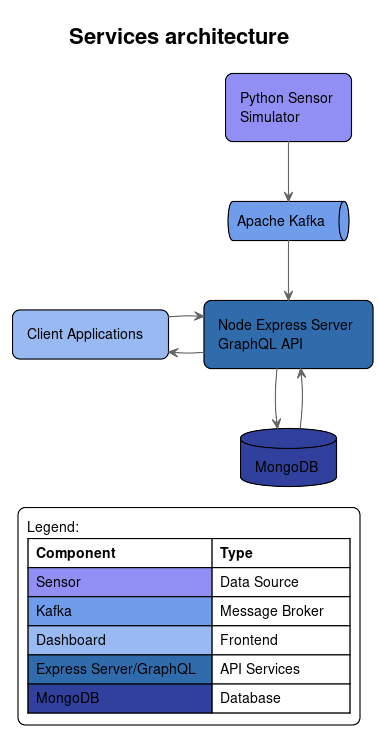
\includegraphics[width=0.5\textwidth]{architecture.png}
  \caption{Architettura generale del sistema}
  \label{fig:architecture}
\end{figure}

Di seguito vengono esplicitate le varie responsabilità per ognuno dei servizi precedentemente elencati.

\begin{itemize}
  \item Sensor service: questo servizio simula l'esercizio di un insieme di sensori, i quali registrano,
        con cadenza regolare, le misurazioni della qualità dell'aria. Ogni sensore è provvisto di un id univoco,
        un nome, una posizione geografica (le coordinate della sua collocazione) ed un indirizzo \acrshort{ip}.
        Tali misurazioni vengono inviate al broker dei messaggi in modo che vengano poi trasmesse ai servizi in ascolto.
  \item Broker service: questo servizio dispone di un canale di comunicazione logico (topic)
        dove vengono pubblicate e consumate le informazioni. Nel canale vengono accodate le misurazioni
        ottenute dai sensori, le quali sono poi consumate dal servizio del server \acrshort{api},
        per la loro gestione ed erogazione.
  \item \acrshort{api} service: questo servizio consuma dal broker le misurazioni, le salva
        sul database non relazione e le rende disponibili attraverso \acrshort{api}.
  \item Dashboard service: questo servizio fornisce un'interfaccia grafica tramite cui è possibile consultare
        la mappa interattiva, aggiornata in tempo reale con i dati forniti dal server \acrshort{api}, e le relative
        tabelle.
  \item Database service: questo servizio si occupa di salvare in modo persistente le misurazioni
        registrate dai sensori, permettendo future interrogazioni sui dati storici.
\end{itemize}

\section{Sensor service}

In questa sezione verrà descritto il servizio che simula il sensore e la relativa generazione di misurazioni fittizie
sulla qualità dell'aria.

\subsection{Modello sensore}

Il sensore è dotato di un insieme di proprietà specifiche che ne determinano il funzionamento.
Queste proprietà sono:

\begin{itemize}
  \item Id (\texttt{sensor\_id}): stringa, identificatore univoco del sensore.
  \item Nome (\texttt{name}): stringa, nome del sensore.
  \item Posizione (\texttt{location}): oggetto, posizione in cui è collocato il sensore.
        Si tratta di un oggetto composto dal tipo (in questo caso \texttt{Point}) e dalle coordinate,
        longitudine e latitudine, ambo valori numerici a virgola mobile (\texttt{double}).
  \item \acrshort{ip} (\texttt{ip}): stringa, indirizzo ip del sensore.
  \item Attivo (\texttt{active}): booleano, indica se il sensore è attivo (\texttt{true})
        oppure no (\texttt{false}).
  \item Ultima misurazione (\texttt{last\_seen}): data, ultima volta che il sensore ha registrato una misurazione.
        \label{lst:sensors-properties}
\end{itemize}

\subsection{Generazione pseudo-misurazioni}

La classe \texttt{AirQualitySensor} è dotata di un metodo \texttt{generate\_reading} che produce misurazioni simulate.
Ad ogni sensore viene fornita la configurazione presentata in lista~\ref{lst:sensor-config} per la generazione
delle misurazioni.

\begin{lstlisting}[caption={Configurazione sensore}, label=lst:sensor-config]
  SENSOR_CONFIG = {
    'sampling_rate': 10,            # seconds (def. 60)

    # Sensor ranges
    'temperature_range': (-15, 35), # Celsius degrees
    'humidity_range': (30, 100),    # %
    'pressure_range': (980, 1020),  # hPa
    'voc_range': (0, 3),            # ppm
    'co2_range': (400, 2000),       # ppm
    'pm25_range': (0, 150),         # micrograms/m^3
    'pm10_range': (0, 300),         # micrograms/m^3
    'no2_range': (0, 200),          # micrograms/m^3
    'o3_range': (0, 200),           # micrograms/m^3
    'so2_range': (0, 300),          # micrograms/m^3
  }
\end{lstlisting}

Per mantenere coerenza nei dati e evitare valori troppo discordanti, ogni nuova misurazione generata dal sensore
si basa sulla lettura precedente (quando disponibile) e si discosta da essa di una percentuale compresa tra
l'1\% e il 5\%.

Parte del codice Python utilizzato per la generazione di queste misurazioni simulate è riportato
nella lista~\ref{lst:generate-reading} che segue.

\begin{lstlisting}[caption={Metodo per la generazione di pseudo-misurazioni}, label=lst:generate-reading]
  def generate_reading(self):
    """Generate a realistic sensor reading with some correlation between values
    and small random changes (1-5%) from previous readings if available"""

    # Apply random change of 1-5% to previous values
    def random_change(value):
        percent_change = random.uniform(0.01, 0.05)  # 1-5%
        direction = random.choice([-1, 1])  # Increase or decrease
        return value * (1 + direction * percent_change)

    # Gas pollutants with random changes #

    # PM2.5 and PM10 with correlation maintained
    pm25 = random_change(self.last_reading['pm25'])
    pm25 = np.clip(pm25, *self.config['pm25_range'])

    pm10 = max(pm25 + random_change(self.last_reading['pm10'] - self.last_reading['pm25']), pm25)
    pm10 = np.clip(pm10, pm25, self.config['pm10_range'][1])

    # Nitrogen dioxide levels
    no2 = random_change(self.last_reading['no2'])
    no2 = np.clip(no2, *self.config['no2_range'])

    # Ozone levels
    o3 = random_change(self.last_reading['o3'])
    o3 = np.clip(o3, *self.config['o3_range'])

    # Sulfur dioxide levels
    so2 = random_change(self.last_reading['so2'])
    so2 = np.clip(so2, *self.config['so2_range'])
\end{lstlisting}

\subsection{Distribuzione sensori}
\label{subsection:sensor-distribution}

La scelta dei sensori è stata fatta relativamente ai punti di maggiore traffico, quali le intersezioni stradali
fra le arterie principali e le strade secondarie. Bologna presenta una moltitudine di semafori, luogo dove veicoli
fermi in attesa tendono a creare punti di maggiore concentrazione di inquinanti. Come anticipato precedentemente
con la query \ref{lst:overpass-query}, sono stati estrapolati tutti i punti che rappresentano un'intersezione
stradale di questo tipo. Data l'elevata densità di posizioni rilevate, è stata applicata una selezione sistematica
per mantenere un singolo punto per ogni intervallo di spazio regolare.
Questa selezione ha permesso anche di gestire le situazioni di affollamento, tipiche di rotonde,
nelle quali ogni svincolo è rappresentato come un incrocio, e di centri abitati, nei quali la concentrazione
di queste intersezioni risulta più elevato.

Nelle immagini \ref{fig:sensors-before} e \ref{fig:sensors-after} viene mostrato come, partendo da un dataset
consistente di punti, questi siano stati poi filtrati secondo i criteri precedentemente esposti.
È stata implementata una griglia di campionamento con spaziatura di 250 metri, parametro calibrato
sperimentalmente per ottenere una densità ottimale di punti. Per fare ciò è stata realizzata una pagina dedicata
allo scopo, dato che si tratta di un processo che può essere riprodotto
cambiando la distanza fra i punti tramite input numerico.
0La pagina presenta una parte iniziale dove è possibile scegliere la città (nel nostro caso Bologna) e lo spazio
minimo fra un sensore e l'altro. Viene anche indicata la query di estrazione,
la stessa citata in precedenza nella lista~\ref{lst:overpass-query}.
Questa parte d'intestazione è riportata nell'immagine~\ref{fig:sensors-heading}, dove si possono notare gli elementi
citati.

\begin{figure}[H]
  \centering
  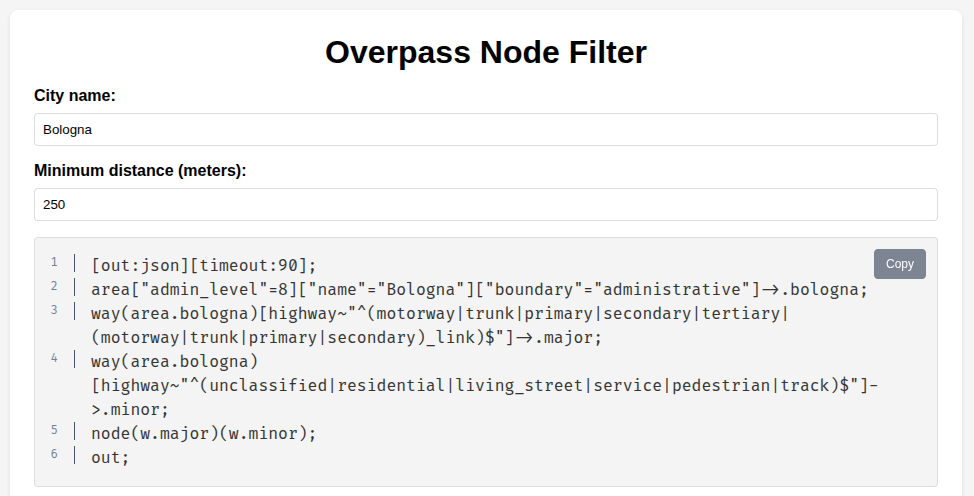
\includegraphics[width=0.65\textwidth]{sensors/00_heading.png}
  \caption{Intestazione pagina}
  \label{fig:sensors-heading}
\end{figure}

Sotto di essa, è disponibile la mappa che mostra i nodi risultanti dalla query.
Tali nodi vengono disposti su 3 livelli, che sono: nodi originali, nodi filtrati e nodi differenza.
I primi, quelli originali (in rosso, immagine~\ref{fig:sensors-before}),
sono ottenuti direttamente dalla query ~\ref{formula:sensors-original}.
I secondi, quelli filtrati (in blu, immagine~\ref{fig:sensors-after}), sono il risultato del trattamento effettuato
su di essi, dato dall'elezione di un solo nodo ogni 250 metri ~\ref{formula:sensors-filtered}.
Gli ultimi infine, quelli di differenza (in verde, immagine~\ref{fig:sensors-difference}),
sono semplicemente i nodi originali
meno quelli filtrati ~\ref{formula:sensors-difference}.
La richiesta viene effettuata nel momento in cui viene cliccato il pulsante di invio, che riporta la
dicitura \textit{"Submit request"}. Si tratta di una chiamata POST
all'indirizzo \url{https://overpass-api.de/api/interpreter"}, il quale restituisce un \acrshort{json} in caso di
esito positivo.

\definecolor{sensors-original}{HTML}{e74c3c}
\definecolor{sensors-filtered}{HTML}{3498db}
\definecolor{sensors-difference}{HTML}{27ae60}

\begin{align}
  \textcolor{sensors-original}{O}   & = \text{insieme degli elementi originali} \label{formula:sensors-original}                                                                                                                            \\
  \textcolor{sensors-filtered}{F}   & = \text{sottoinsieme filtrato, dove } \textcolor{sensors-filtered}{F}\subseteq \textcolor{sensors-original}{O} \label{formula:sensors-filtered}                                                       \\
  \textcolor{sensors-difference}{D} & = \textcolor{sensors-original}{O} \setminus \textcolor{sensors-filtered}{F} = \{x \in \textcolor{sensors-original}{O} : x \notin \textcolor{sensors-filtered}{F}\} \label{formula:sensors-difference}
\end{align}

\newpage

\begin{figure}[H]
  \centering

  \begin{subfigure}{\textwidth}
    \centering
    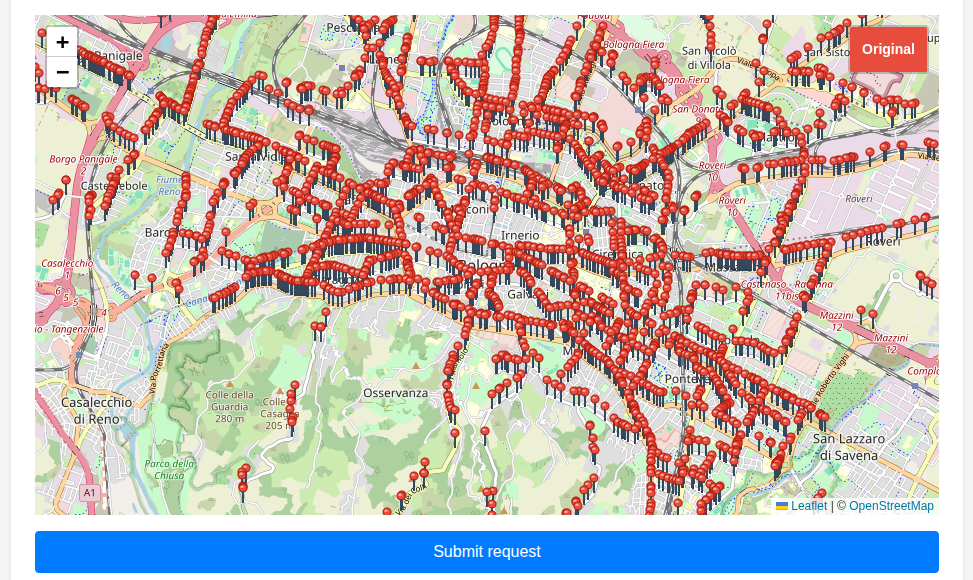
\includegraphics[width=0.85\textwidth]{sensors/01_original.png}
    \caption{Risultato originale della query}
    \label{fig:sensors-before}
  \end{subfigure}

  \hfill
  \begin{subfigure}{\textwidth}
    \centering
    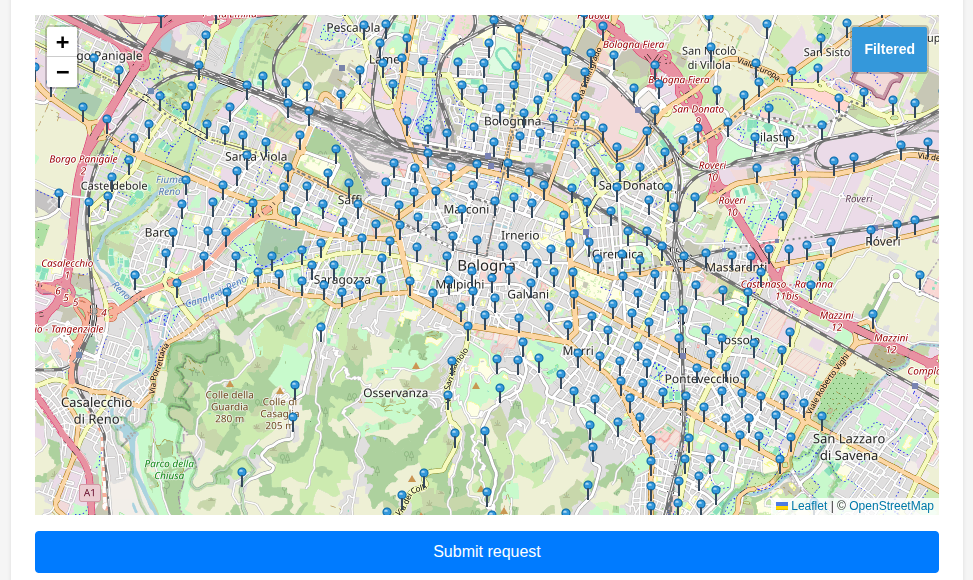
\includegraphics[width=0.85\textwidth]{sensors/02_filtered.png}
    \caption{Punti filtrati finali}
    \label{fig:sensors-after}
  \end{subfigure}


  \hfill
  \begin{subfigure}{\textwidth}
    \centering
    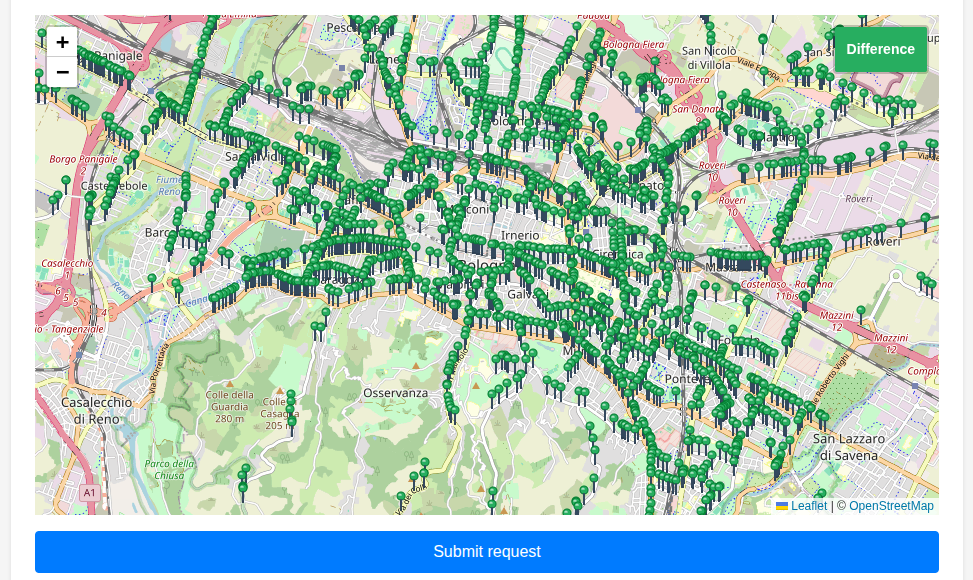
\includegraphics[width=0.85\textwidth]{sensors/03_difference.png}
    \caption{Punti di differenza}
    \label{fig:sensors-difference}
  \end{subfigure}

  \caption{Acquisizione punti delle intersezioni stradali}
\end{figure}

\newpage

Come ultimo elemento, la parte finale della pagina, esposta nell'immagine~\ref{fig:sensors-footer},
riporta le statistiche quali il numero di sensori originale,
il numero di sensori filtrati e la riduzione espressa come percentuale.
Premendo il pulsante con scritto \textit{"Download filtered \acrshort{json}"} è possibile scaricare il
\acrshort{json} dei sensori filtrati ottenuti. Tale \acrshort{json} presenta i sensori usati per popolare la mappa
dell'applicazione principale.

\begin{figure}[H]
  \centering
  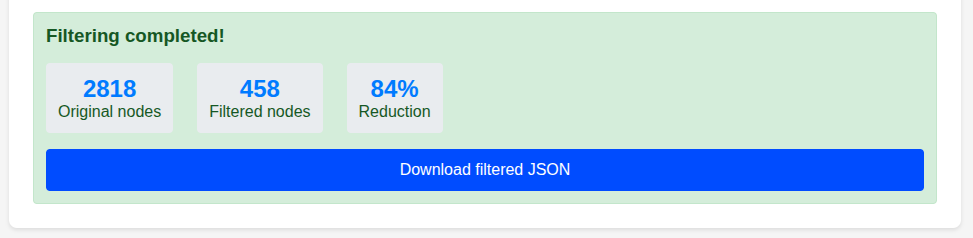
\includegraphics[width=\textwidth]{sensors/03_footer.png}
  \caption{Piè di pagina}
  \label{fig:sensors-footer}
\end{figure}

\section{Broker service}

In questa sezione verrà descritto il servizio di message broker rispetto alle gestione delle misurazioni fittizie
generate dai sensori e consumate dal server.

\subsection{Architettura del Sistema}

Il sistema utilizza Apache Kafka come message broker per gestire il flusso di dati
tra i sensori Python e il server Node.js. È configurato in modalità \acrfull{kraft}, che elimina la dipendenza
da Apache ZooKeeper per la gestione dei metadati del cluster.
L'utilizzo Apache Kafka in questa configurazione porta diversi benefici significativi al sistema.
Innanzitutto, la piattaforma permette di elaborare i dati provenienti dai sensori in modo asincrono e con prestazioni
elevate, garantendo un throughput alto anche con volumi considerevoli di informazioni.
Un altro aspetto vantaggioso è che sensori e server possono funzionare in completa autonomia l'uno dall'altro,
senza dipendenze dirette che potrebbero creare colli di bottiglia o punti di failure.
Questa indipendenza si traduce anche in una maggiore flessibilità del sistema: è possibile aggiungere nuovi sensori
alla rete senza dover apportare modifiche al codice del consumer, rendendo l'architettura facilmente scalabile.
La persistenza dei dati rappresenta un ulteriore punto di forza: tutti i messaggi vengono conservati nei log di Kafka
per un periodo di tempo configurabile secondo le esigenze specifiche del progetto.
Questo significa che le informazioni non vanno perse anche in caso di interruzioni temporanee.
Infine, Kafka gestisce automaticamente aspetti critici come le riconnessioni in caso di problemi di rete e le procedure
di recovery, riducendo significativamente la complessità operativa e aumentando l'affidabilità complessiva del sistema.

\paragraph{Produzione dei Messaggi}

I sensori Python generano misurazioni simulate della qualità dell'aria e le incapsulano
in un \acrshort{json} per poi pubblicale sul topic Kafka \texttt{measurements}, connettendosi
al broker tramite l'indirizzo interno \texttt{kafka:9092}.

\paragraph{Consumo dei Messaggi}

Il server Node.js agisce come consumer Kafka, rimanendo in ascolto continuo sul topic \texttt{measurements},
ricevendo le misurazioni simulate della qualità dell'aria registrate in esso. Su tali misurazioni viene effettuato
il parsing \acrshort{json} e la validazione dei dati ricevuti. Se le misurazioni ottenute sono valide,
vengono salvate nel database MongoDB ed inoltrate ai client web tramite WebSocket.

\paragraph{Health Check}

Il container Kafka include un health check che verifica periodicamente la disponibilità del broker
attraverso il comando \texttt{kafka-topics.sh}, con parametri di retry configurabili quali:
intervallo di controllo (30 secondi), timeout (15 secondi), numero di tentativi (10) e periodo di avvio (30 secondi).

\section{\acrshort{api} service}

In questa sezione verrà descritto il servizio \acrshort{api} che riceve le misurazioni simulate della qualità dell'aria
dal broker di messaggi, le trasforma ed eroga ai client che lo interrogano.

\subsection{Architettura del Server}

Il server Node.js implementa un'architettura basata su Express.js che espone \acrshort{api} \acrshort{rest}ful
per l'accesso ai dati delle misurazioni ambientali.
Il server integra diverse tecnologie per fornire un servizio completo.
Express.js gestisce le richieste \acrshort{http} come framework web principale,
mentre MongoDB si occupa della persistenza dei dati attraverso un database NoSQL flessibile e scalabile.
Apache Kafka funge da sistema di messaggistica per il consumo continuo dei dati sensoriali,
garantendo un flusso affidabile delle informazioni.
Socket.IO abilita la comunicazione WebSocket per fornire aggiornamenti in tempo reale ai client connessi.
La configurazione \acrshort{cors} completa l'architettura consentendo richieste cross-origin sicure e controllate,
necessarie per il corretto funzionamento dell'applicazione web distribuita.

\subsection{Endpoint Disponibili}

Di seguito verranno elencati gli endpoint disponibili esposti dalle \acrshort{api}.
Tutti gli endpoint di seguito elencati restituiscono un \acrshort{json} ed un codice di stato \acrshort{http} che può
essere \texttt{200 OK} in caso di successo o \texttt{500 Internal Server Error} in caso di errore.

\subsubsection{Health Check - \texttt{GET /health}}

Endpoint per il monitoraggio dello stato del servizio.
Verifica la disponibilità del server e restituisce lo stato operativo.
Risponde con un semplice \acrshort{json} con lo status ed il tempo di attività,
come da esempio~\ref{lst:api-health-example}.

\begin{lstlisting}[caption={Risposta di sucesso per endpoint \texttt{health}}, label=lst:api-health-example]
  {
    "status":"healthy",
    "timestamp":"2025-08-30T13:58:44.198Z",
    "uptime":39.198012656
  }
\end{lstlisting}

\subsubsection{Recupero Misurazioni - \texttt{GET /api/measurements}}

Endpoint per il recupero delle misurazioni ambientali con supporto per filtri e paginazione.
Restituisce le misurazioni archiviate nel database con possibilità di filtraggio per sensore e intervallo temporale.

È possibile utilizzare dei parametri opzionali di query, quali
\texttt{sensorId} come identificativo del sensore specifico,
data di inizio \texttt{startDate} e fine \texttt{endDate} del periodo di misurazione (in formato \acrshort{iso} 8601).
Se specificato \texttt{sensorId}, filtra per sensore specifico,
mentre se specificati \texttt{startDate} e \texttt{endDate}, filtra per intervallo temporale.
Le misurazioni in risposta sono in ordine crescente per timestamp e con limite massimo di 1000 record per richiesta.

Un esempio di risposta di successo è riportato nella lista~\ref{lst:api-measurements-example}
\begin{lstlisting}[caption={Risposta di sucesso per endpoint \texttt{measurements}},label=lst:api-measurements-example]
[
  {
    "_id":"68a4def8c82270d8766481f6",
    "sensor_id":"SENSOR00436",
    "timestamp":"2025-08-19T22:30:48.494Z",
    "temperature":2.64,
    "humidity":75.87,
    "pressure":1019.63,
    "voc":0.647,
    "co2":400,"pm25":55.43,
    "pm10":177.75,
    "no2":132.4,
    "o3":65.45,
    "so2":35.95,
    "__v":0
  },
  ...
]
\end{lstlisting}

\subsubsection{Lista Sensori - \texttt{GET /api/sensors}}

Endpoint per il recupero dell'elenco completo dei sensori registrati nel sistema.
Restituisce tutti i sensori configurati con le relative informazioni di localizzazione e configurazione.
È possibile utilizzare come parametro opzionale di query \texttt{sensorId} come identificativo del sensore specifico,
estraendo il solo sensore indicato (se disponibile).

Un esempio di risposta di successo è riportato nella lista~\ref{lst:api-sensors-example}
\begin{lstlisting}[caption={Risposta di sucesso per endpoint \texttt{sensors}},label=lst:api-sensors-example]
[
  {
    "location": { "type": "Point", "coordinates": [11.3482468, 44.4856545] },
    "_id": "68a4b0b50bb78efcdfbaa8b9",
    "sensor_id": "SENSOR00001",
    "name": "d0d54bf349674398",
    "ip": "192.168.0.1",
    "active": true,
    "last_seen": "2025-08-30T10:21:32.252Z"
  },
  ...
]
\end{lstlisting}

\subsubsection{Ultima Misurazione - \texttt{GET /api/latest}}

Endpoint per il recupero della misurazione più recente nel sistema.
Restituisce l'ultima misurazione registrata, ordinata per timestamp decrescente.

Un esempio di risposta di successo è riportato nella lista~\ref{lst:api-latest-example}
\begin{lstlisting}[caption={Risposta di sucesso per endpoint \texttt{latest}},label=lst:api-latest-example]
{
  "_id":"68b421c342b53a3e45108d73",
  "sensor_id":"SENSOR00238",
  "timestamp":"2025-08-30T12:19:47.467Z",
  "temperature":15.42,
  "humidity":32.71,
  "pressure":980,
  "voc":1.937,
  "co2":417.1,
  "pm25":16.76,
  "pm10":131.12,
  "no2":57.75,
  "o3":130.33,
  "so2":112.44,
  "__v":0
}
\end{lstlisting}

\section{Dashboard service}

Questa sezione sarà dedicata alla descrizione dell'applicazione frontend sviluppata per il progetto AirQualityInsight.
L'esposizione verrà articolata in due parti distinte: nella prima sottosezione verrà presentata
l'interfaccia utente e verranno illustrate le scelte progettuali che hanno guidato la definizione del design,
mentre nella seconda sottosezione verrà fornita una descrizione dettagliata dell'implementazione
tecnica dell'applicazione.

\subsection{Design e architettura dell'interfaccia}

In questa sottosezione verrà illustrata l'interfaccia dell'applicazione e verranno esaminate le scelte progettuali
che hanno determinato la sua configurazione.
La progettazione dell'interfaccia è stata condotta tenendo conto degli obiettivi e delle funzionalità stabilite
durante la fase di analisi, nonché dello studio dello stato dell'arte delle applicazioni attualmente
disponibili nel settore.
Il processo di design dell'interfaccia grafica è stato orientato dai seguenti principi guida:
\begin{itemize}
  \item i requisiti funzionali e non funzionali definiti rispettivamente nelle sottosezioni
        \ref{subsec:requisiti-funzionali} e \ref{subsec:requisiti-non-funzionali}
  \item l'approccio mobile-first
  \item l'adozione del principio KISS, orientando l'interfaccia verso uno stile minimalista che privilegia strumenti
        di comunicazione non testuali, quali icone, elementi cromatici e simboli grafici
  \item l'analisi dello stato dell'arte delle applicazioni per il monitoraggio della qualità dell'aria,
        riportata nel capitolo \ref{chapter:first}: si è scelto di mantenere continuità
        con le applicazioni esistenti per il monitoraggio della qualità dell'aria, al fine di offrire agli utenti
        un'esperienza familiare e sfruttare le soluzioni progettuali già consolidate
\end{itemize}
L'architettura dell'interfaccia è stata strutturata mediante la suddivisione dei componenti
in tre categorie principali, classificate in base alla loro collocazione spaziale e alle rispettive funzionalità,
sia individuali che sinergiche con gli altri elementi del sistema.
Nei paragrafi seguenti verranno presentate le categorie identificate e i rispettivi componenti costitutivi.

\subsection{Implementazione}

In questa sottosezione verrà approfondita nel dettaglio l'implementazione dell'applicazione web di AirQualityInsight.
Tale applicazione è stata realizzata basandosi principalmente su Vue e Leaflet.
Nelle seguenti sottosezioni verranno esaminati i componenti dell'applicativo, ognuno dei quali fa riferimento
ad una porzione dell'interfaccia utente.

\paragraph{Intestazione}

La prima parte dell'applicazione web fornisce un'introduzione riguardo lo scopo del progetto e le sue funzionalità.
Nella seguenti immagini, vengono presentate all'utente, dall'alto verso il basso,
una breve descrizione \ref{fig:app-description},
la tabella relativa ai criteri di valutazione della qualità dell'aria \ref{fig:app-eaqi-table},
una guida sintetica sull'utilizzo della pagina \ref{fig:app-guide} ed infine
il metodo di calcolo utilizzato per ottenere l'\acrfull{eaqi} \ref{fig:app-eaqi-calculation}.

\begin{figure}[H]
  \centering
  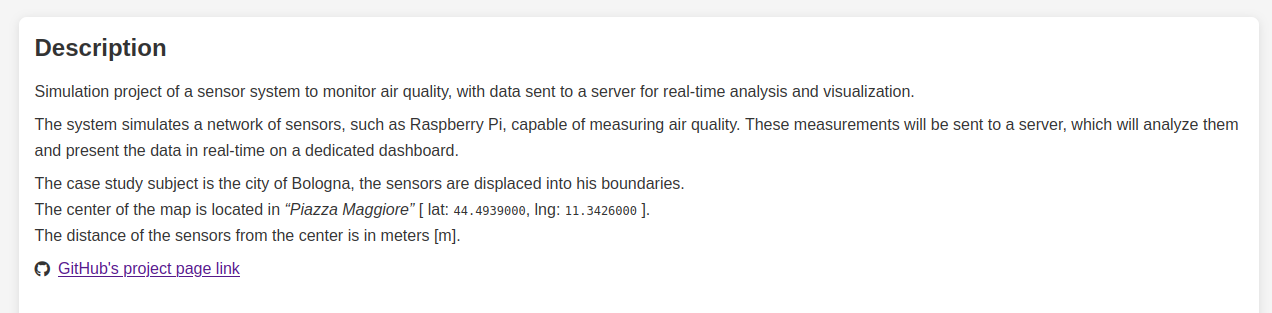
\includegraphics[width=\textwidth]{dashboard/00_disclaimer_description.png}
  \caption{Descrizione}
  \label{fig:app-description}
\end{figure}

\begin{figure}[H]
  \centering
  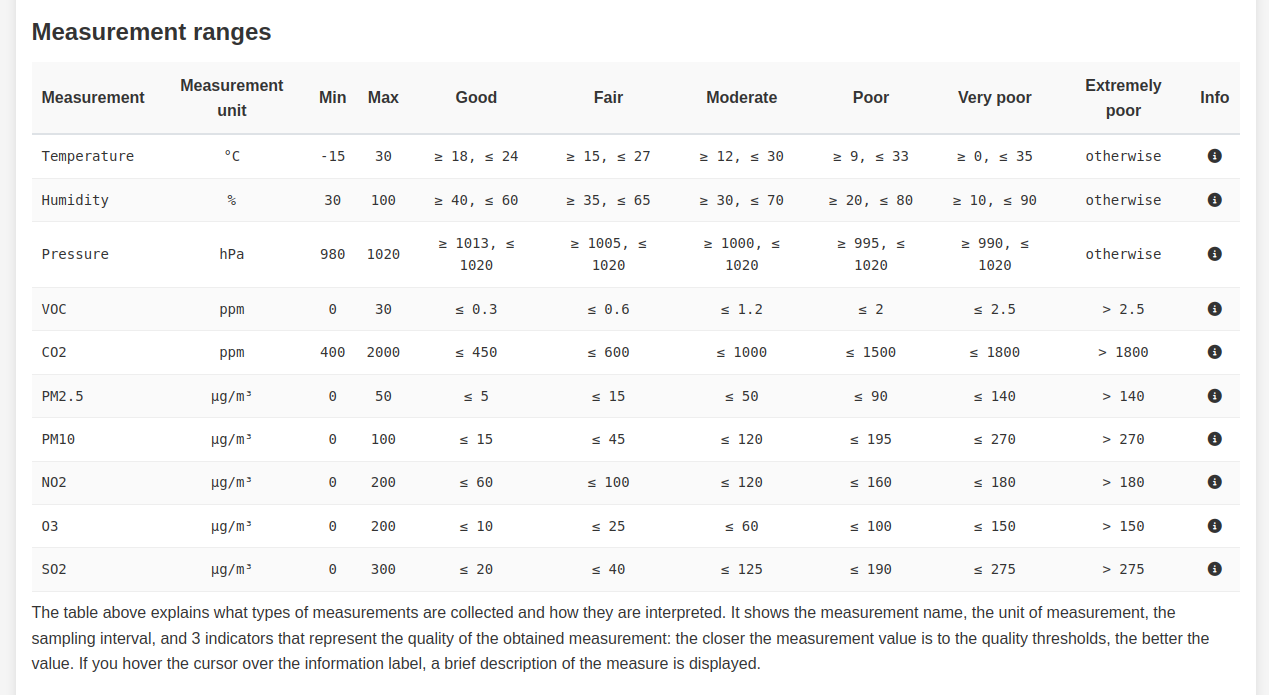
\includegraphics[width=\textwidth]{dashboard/01_table_measurement_ranges.png}
  \caption{Tabella valori riferimento \acrfull{eaqi}}
  \label{fig:app-eaqi-table}
\end{figure}

\begin{figure}[H]
  \centering
  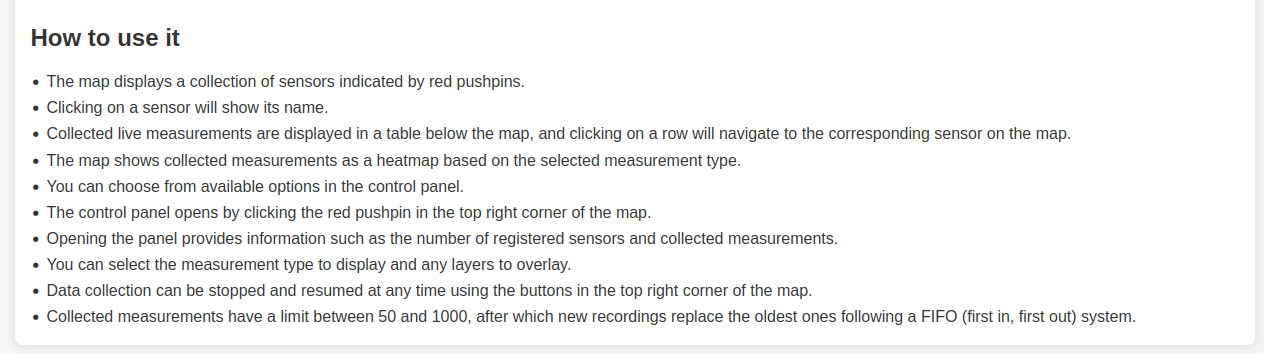
\includegraphics[width=\textwidth]{dashboard/02_disclaimer_how_to_use_it.png}
  \caption{Guida}
  \label{fig:app-guide}
\end{figure}

\begin{figure}[H]
  \centering
  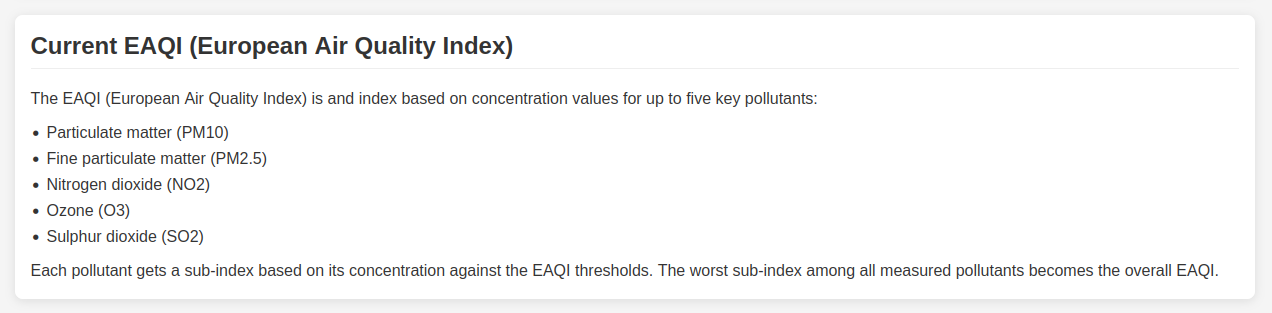
\includegraphics[width=\linewidth]{dashboard/03_disclaimer_eaqi.png}
  \caption{Calcolo \acrfull{eaqi}}
  \label{fig:app-eaqi-calculation}
\end{figure}

\paragraph{Mappa}

Accedendo alla pagina principale, l'utente si trova di fronte a una mappa dettagliata della città di Bologna,
come documentato nell'immagine \ref{fig:app-map-sensors}. La rappresentazione cartografica utilizza un sistema
di simboli colorati per organizzare visivamente le informazioni: i sensori attivi sul territorio
sono contrassegnati da spilli rossi, creando una panoramica immediata della loro distribuzione geografica.
Nel momento in cui viene ricevuta una nuova misurazione, il sensore responsabile viene illuminato nella mappa,
attraverso l'effetto grafico del relativo spillo che lampeggia per un paio di secondi.

Al centro della visualizzazione si trova Piazza Maggiore, simbolo di Bologna, che viene opportunamente evidenziata
con uno spillo blu per distinguerla dagli altri elementi della mappa e fornire un punto di riferimento
costante all'utente, come si può osservare nell'immagine \ref{fig:app-map-center}.

\begin{figure}
  \centering
  \begin{subfigure}{\textwidth}
    \centering
    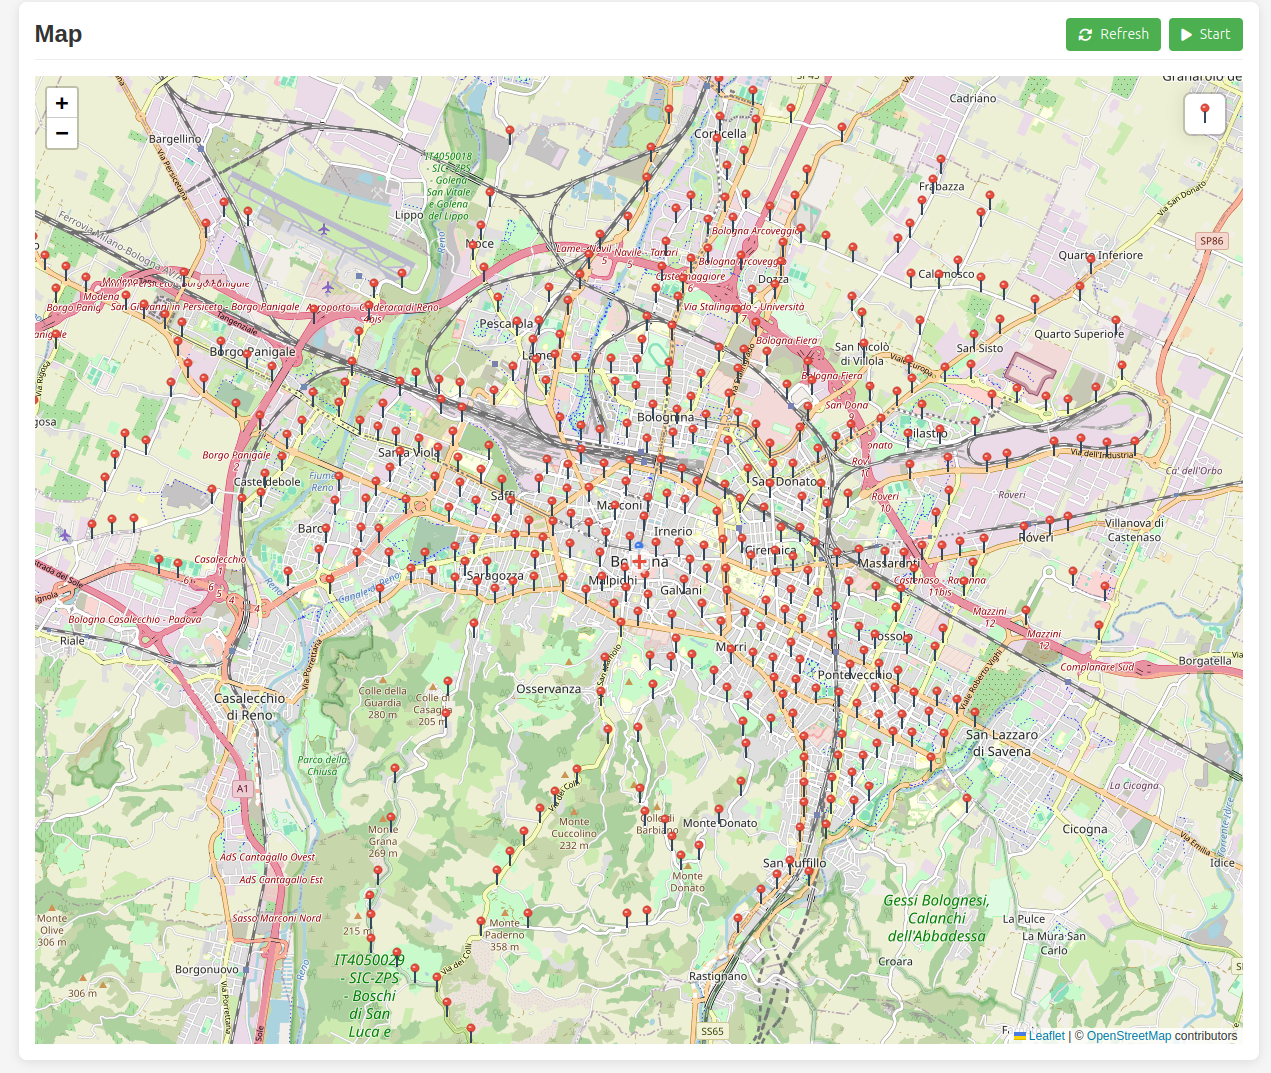
\includegraphics[width=0.95\textwidth]{dashboard/04_map_sensors.png}
    \caption{Mappa principale}
    \label{fig:app-map-sensors}
  \end{subfigure}

  \hfil
  \begin{subfigure}{\textwidth}
    \centering
    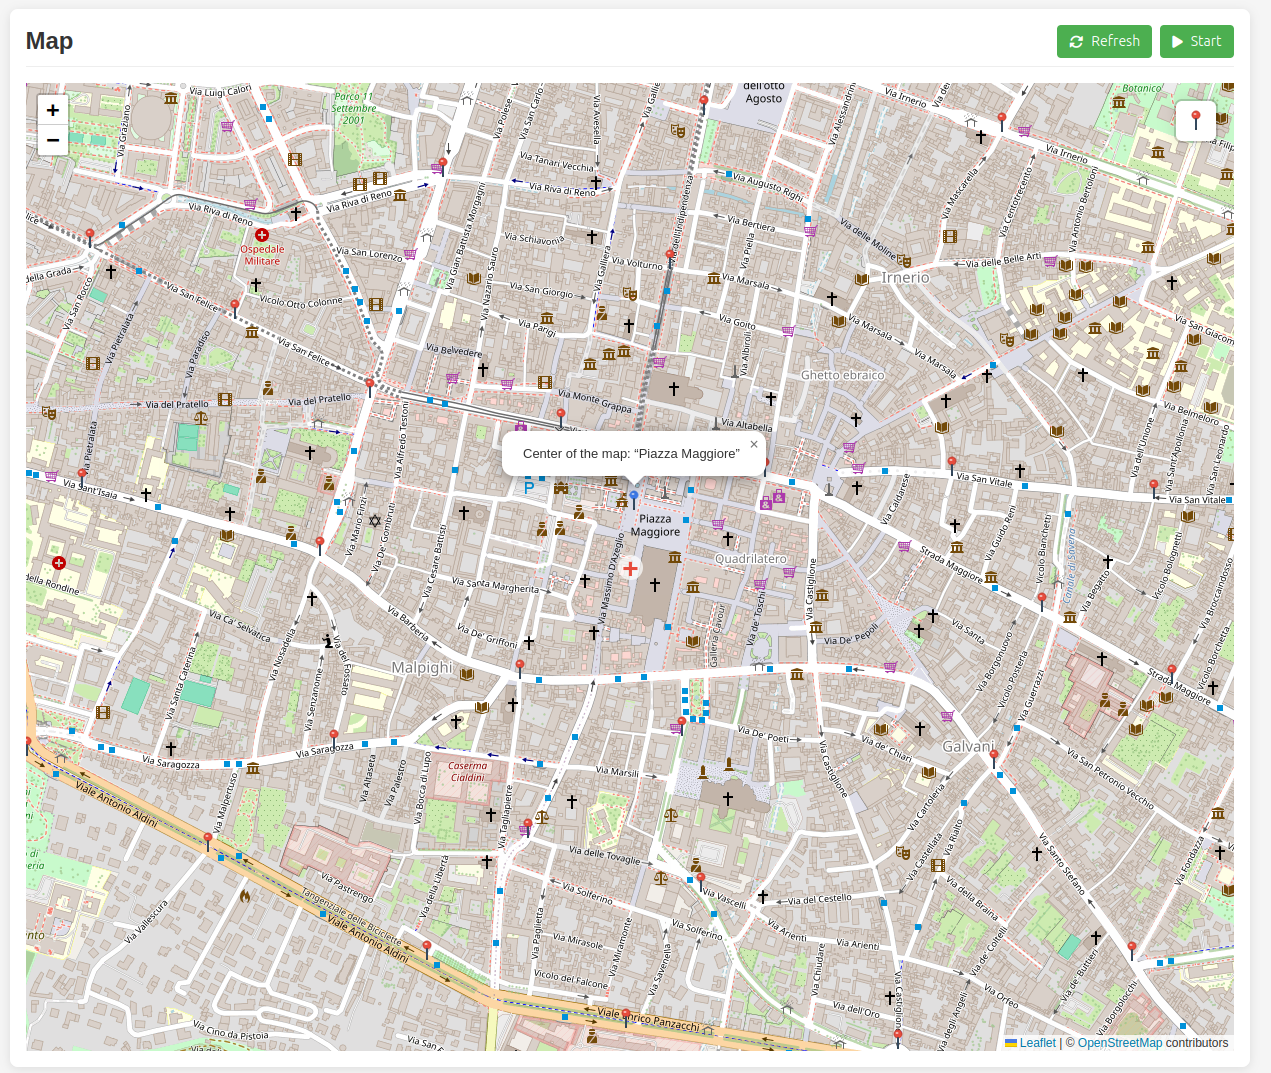
\includegraphics[width=0.95\textwidth]{dashboard/05_map_sensors_center_of_the_map.png}
    \caption{Centro della mappa}
    \label{fig:app-map-center}
  \end{subfigure}
\end{figure}

L'interfaccia cartografica è dotata di diversi controlli interattivi per facilitare la navigazione e la
gestione dei dati.
Sul lato sinistro sono posizionati i pulsanti per aumentare o diminuire lo zoom (\texttt{+} e \texttt{-}) della mappa,
mentre sul lato destro si trovano tre pulsanti: due verdi ed uno bianco avente come icona uno spillo rosso.

Al centro della mappa è presente un indicatore visuale composto da un mirino a croce (\textit{crosshair}) rosso
dentro una cornice circolare bianca. Questo elemento serve come marcatore del punto centrale della
visualizzazione cartografica attuale. Il sistema registra automaticamente le coordinate geografiche associate
alla posizione di questo mirino, conservandole in memoria e rendendole disponibili per la consultazione
da parte dell'utente. Quando l'utente naviga sulla mappa spostando la visualizzazione, le coordinate
del punto centrale vengono aggiornate per mantenere la corrispondenza con la nuova area geografica inquadrata.

Il pulsante verde contrassegnato dalla dicitura \textit{"Start"} rappresenta l'interruttore principale
per attivare o disattivare la ricezione in tempo reale delle misurazioni dai sensori.
All'avvio dell'applicazione, questa funzionalità risulta disabilitata per impostazione predefinita.
Una volta attivata, il sistema inizierà a visualizzare graficamente sulla mappa
i valori ricevuti dai sensori e aggiornerà automaticamente le tabelle informative sottostanti,
come documentato nelle figure \ref{fig:app-tab-last-measurements}, \ref{fig:app-tab-statistics},
\ref{fig:app-tab-system-log} e \ref{fig:app-tab-registered-sensors}.

Il pulsante caratterizzato dall'icona dello spillo rosso attiva l'espansione di un pannello di controllo,
che fornisce informazioni dettagliate sulla mappa attualmente visualizzata e mette a disposizione strumenti
aggiuntivi per l'interazione con l'interfaccia cartografica.
Il pannello di controllo mette a disposizione dell'utente un'ampia gamma di strumenti interattivi, tra cui
informazioni testuali, pulsanti di comando, menu a tendina e un controllo slider orizzontale
(come mostrato nelle figure \ref{fig:map-layer-sensors} e \ref{fig:map-layer-clear}).

Procedendo dall'alto verso il basso, la prima informazione visualizzata concerne il conteggio complessivo
dei sensori presenti sulla mappa. Questo indicatore numerico fornisce un valore globale che comprende tutti
i dispositivi registrati nel sistema, a prescindere dal loro stato operativo attuale. La condizione di funzionamento
viene definita attraverso una proprietà booleana denominata \texttt{status}, che restituisce il valore \texttt{active}
per i sensori operativi. Per un'analisi dettagliata degli attributi di ciascun sensore, è possibile consultare
la tabella documentata nella figura \ref{fig:app-tab-registered-sensors} e nel listato \ref{lst:sensors-properties}.

La sezione successiva presenta un pulsante verde dedicato alla copia delle coordinate geografiche del centro mappa
(corrispondenti alla posizione del mirino). Seguono una serie di pulsanti grigi che consentono
di attivare o disattivare la visualizzazione dei diversi layer cartografici: sensori, demarcazioni territoriali
come le zone di avviamento postale (\acrshort{cap}) (figura~\ref{fig:map-layer-caps}),
quartieri (figura~\ref{fig:map-layer-neighborhoods}),
zone amministrative (figura~\ref{fig:map-layer-zones}) e \acrshort{ztl} (figura~\ref{fig:map-layer-ztl}).

Nella parte inferiore del pannello si trovano ulteriori controlli specializzati: un menu a tendina per la selezione
del tipo di inquinante da visualizzare, uno slider orizzontale per impostare il numero di misurazioni
da registrare (range da 50 a 1000), un indicatore del numero di misurazioni attualmente memorizzate, e un pulsante
rosso con icona cestino per l'eliminazione dei dati registrati. Il sistema implementa un meccanismo di registrazione
delle misurazioni dei sensori basato su una coda (struttura dati \acrshort{fifo}), che garantisce
l'eliminazione automatica delle registrazioni più datate quando viene raggiunta la capacità massima prestabilita,
privilegiando così la conservazione dei dati più recenti.

Conclude l'interfaccia un menu a tendina aggiuntivo per l'attivazione di griglie di riferimento sulla mappa
quali una grigia (figura~\ref{fig:map-grid-gray}), una rossa
(figura~\ref{fig:map-grid-red}) ed una grigia crosshair che divide la mappa
in quattro quarti (figura~\ref{fig:map-grid-crosshair}).

\begin{figure}[H]
  \centering
  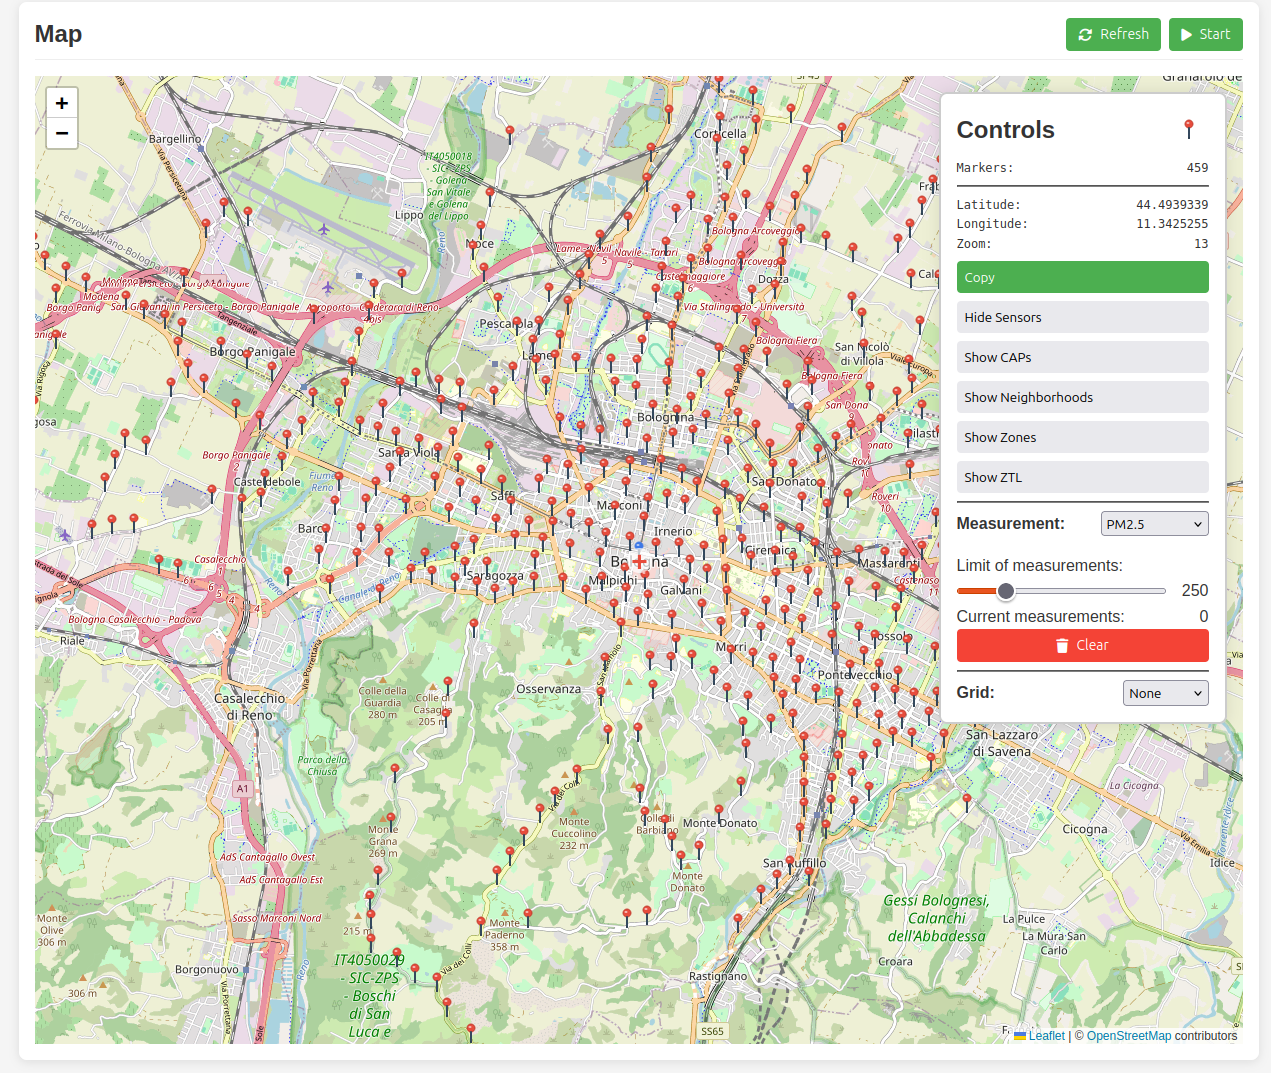
\includegraphics[width=0.95\textwidth]{dashboard/06_map_sensors_controls.png}
  \caption{Pannello controllo espanso con sensori visualizzati}
  \label{fig:map-layer-sensors}

  \hfill

  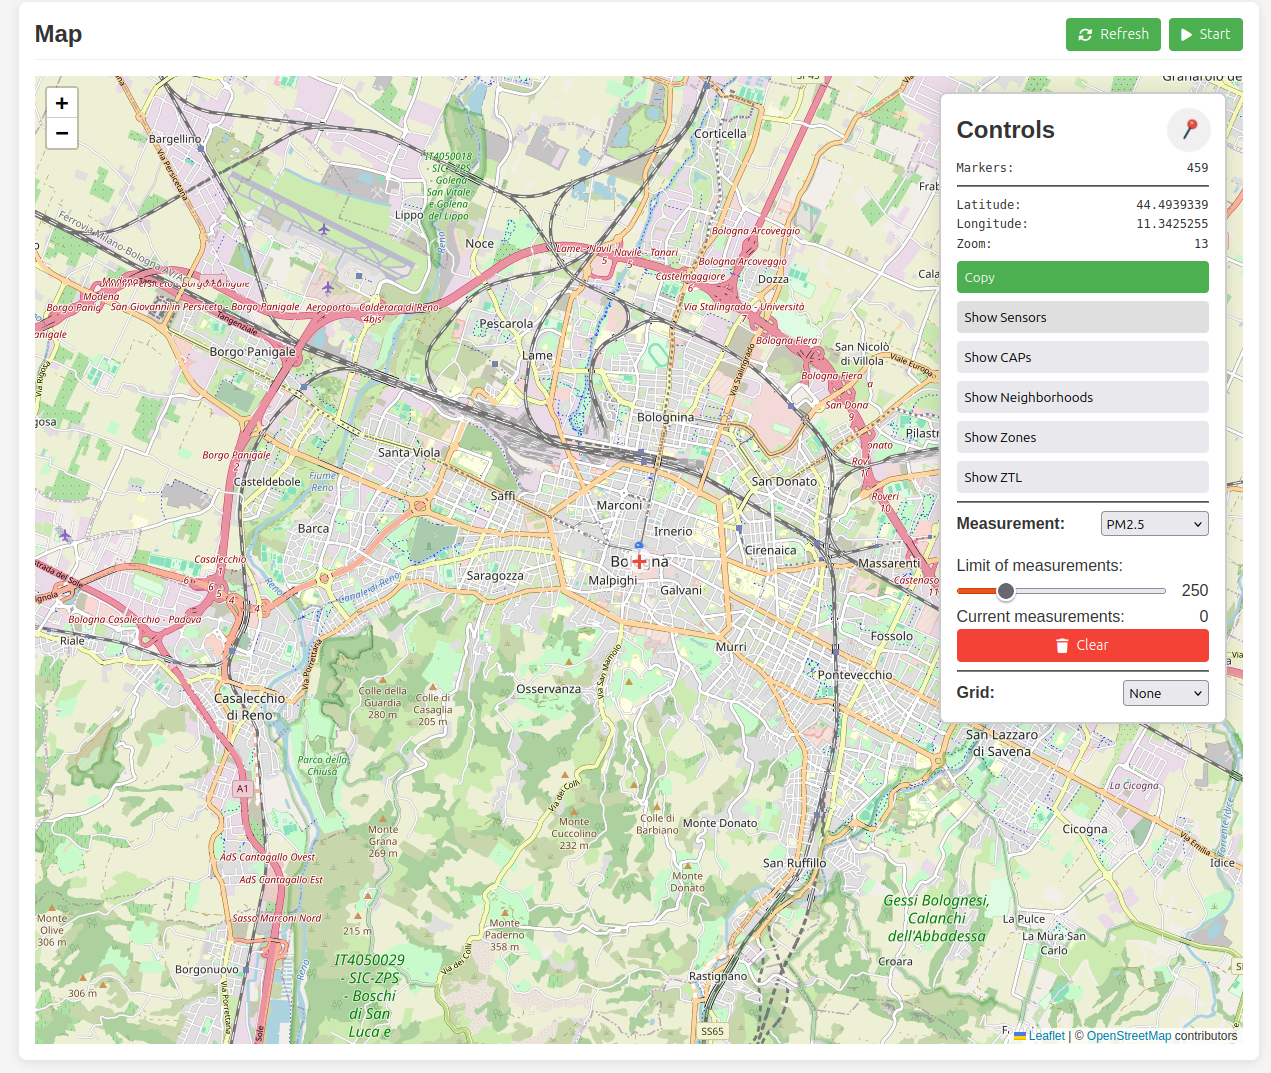
\includegraphics[width=0.95\textwidth]{dashboard/07_map_controls.png}
  \caption{Pannello controllo espanso con sensori nascosti}
  \label{fig:map-layer-clear}
\end{figure}

\newpage

\begin{figure}[H]
  \centering
  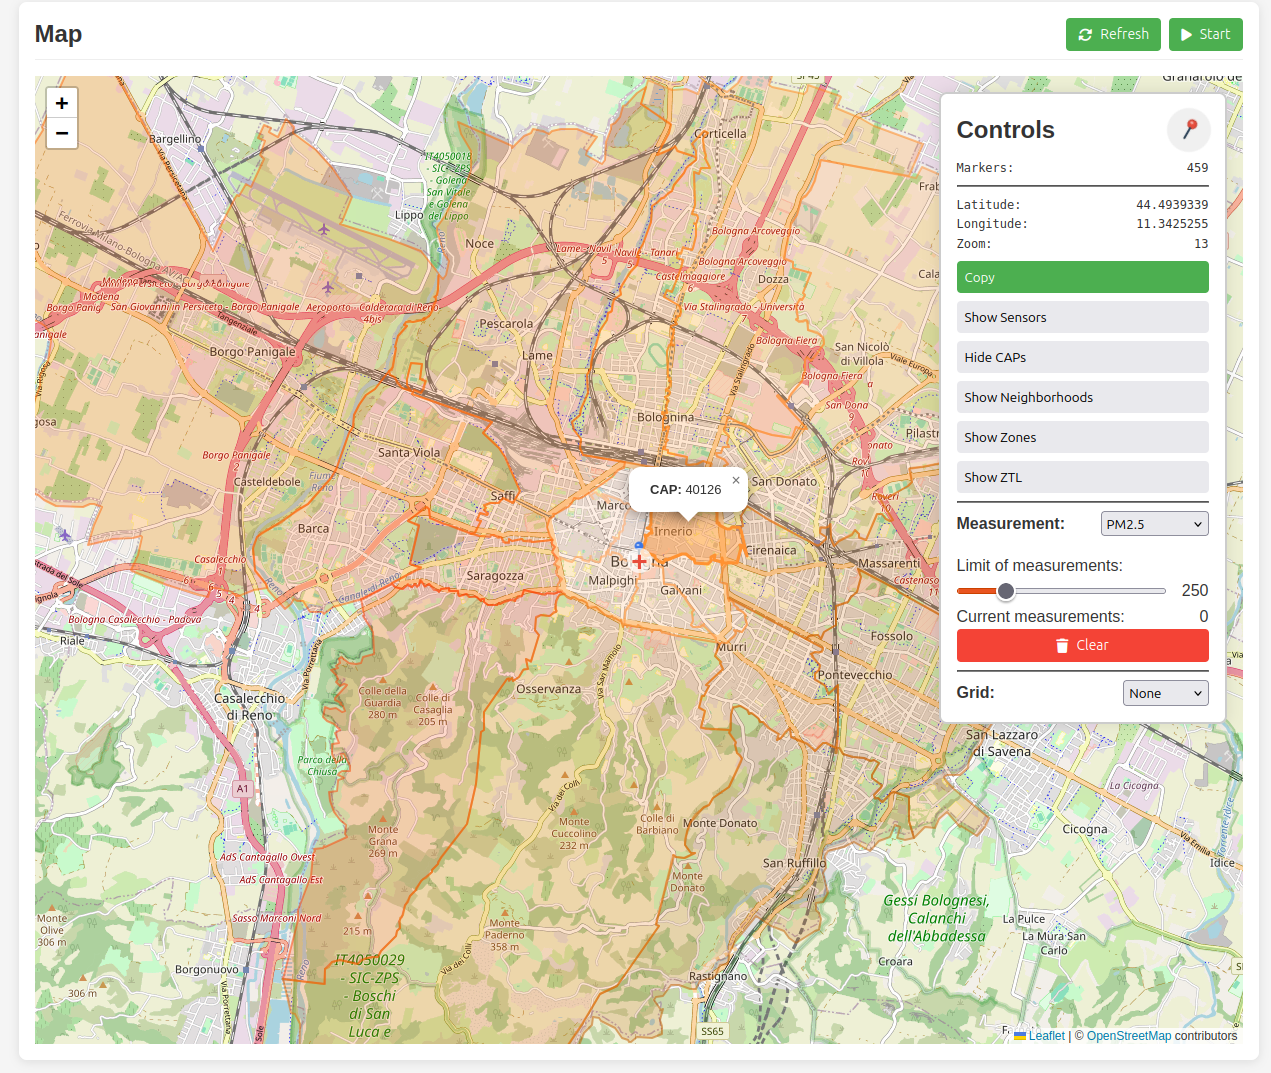
\includegraphics[width=0.95\textwidth]{dashboard/08_map_caps_controls.png}
  \caption{Livello a \acrshort{cap}}
  \label{fig:map-layer-caps}

  \hfill

  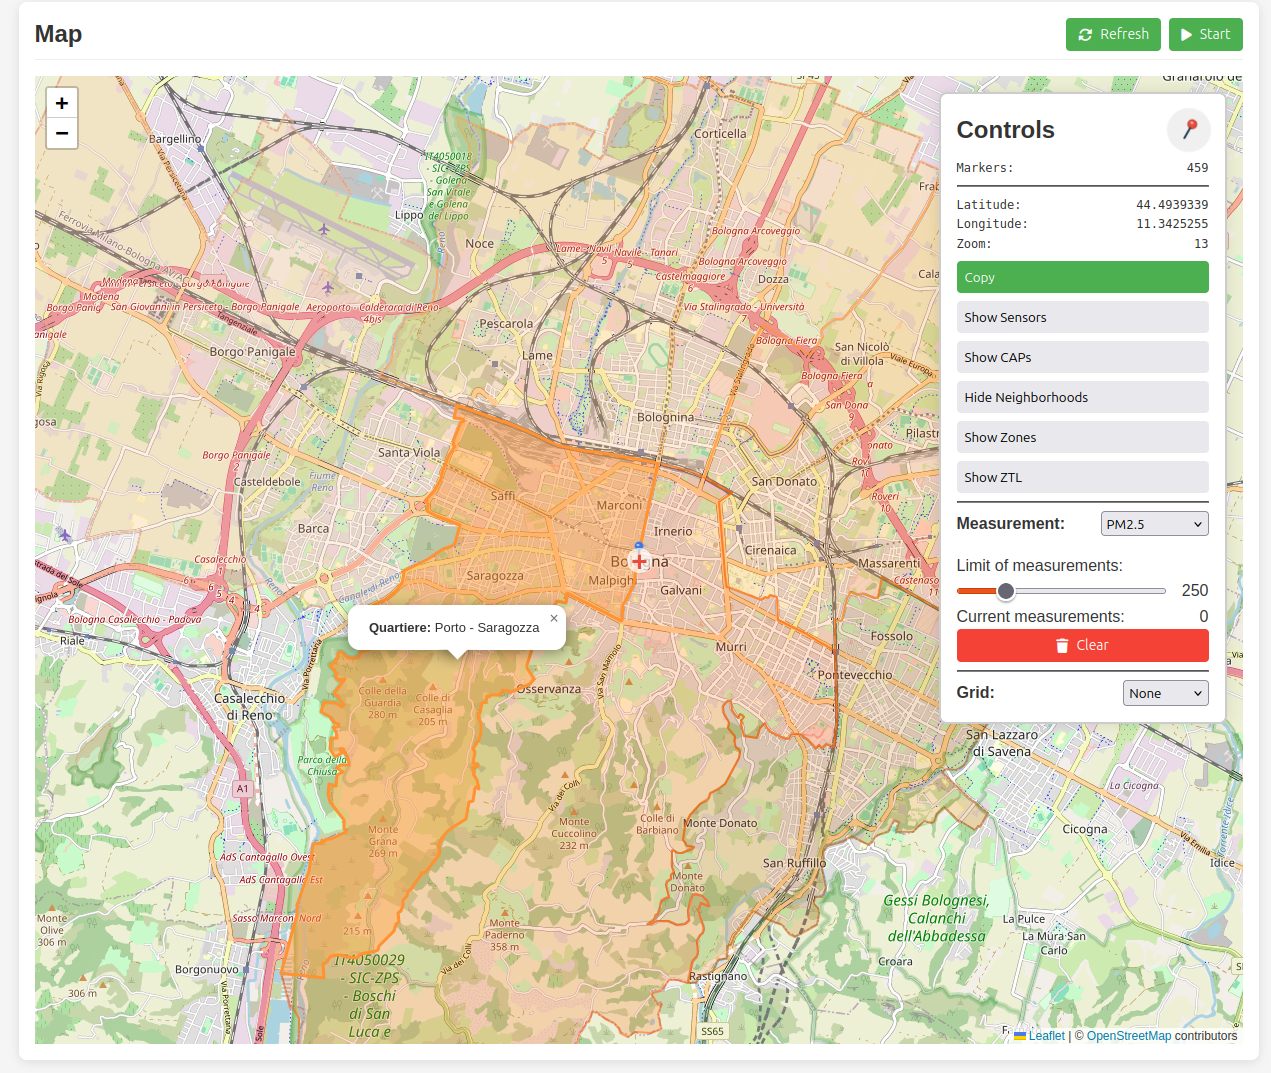
\includegraphics[width=0.95\textwidth]{dashboard/09_map_neighborhoods_controls.png}
  \caption{Livello a quartieri}
  \label{fig:map-layer-neighborhoods}
\end{figure}

\begin{figure}[H]
  \centering
  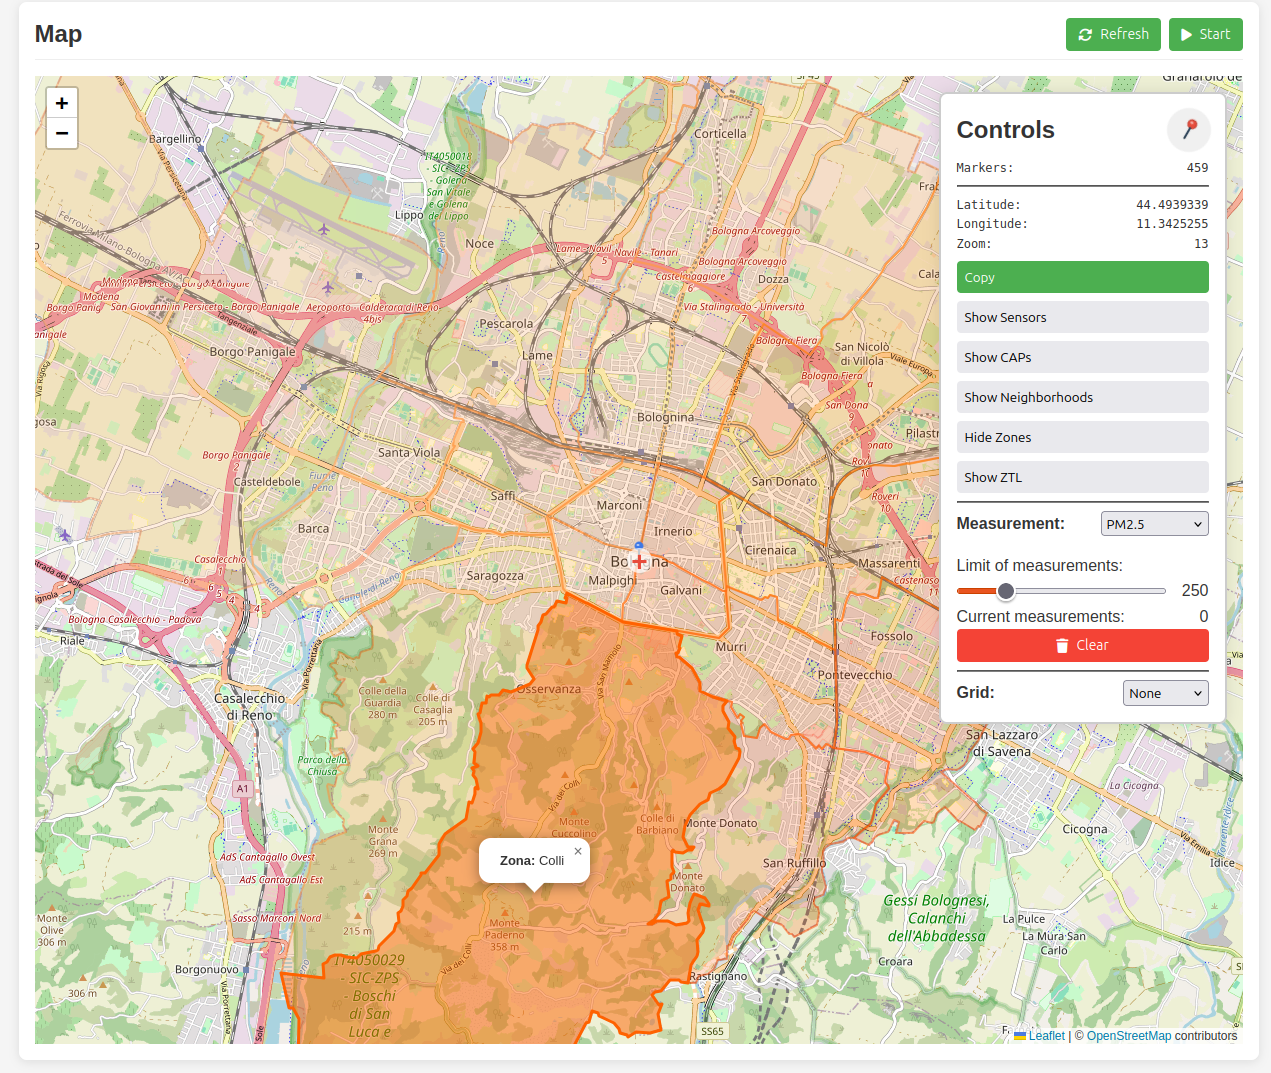
\includegraphics[width=0.95\textwidth]{dashboard/10_map_zones_controls.png}
  \caption{Livello a zone}
  \label{fig:map-layer-zones}

  \hfill

  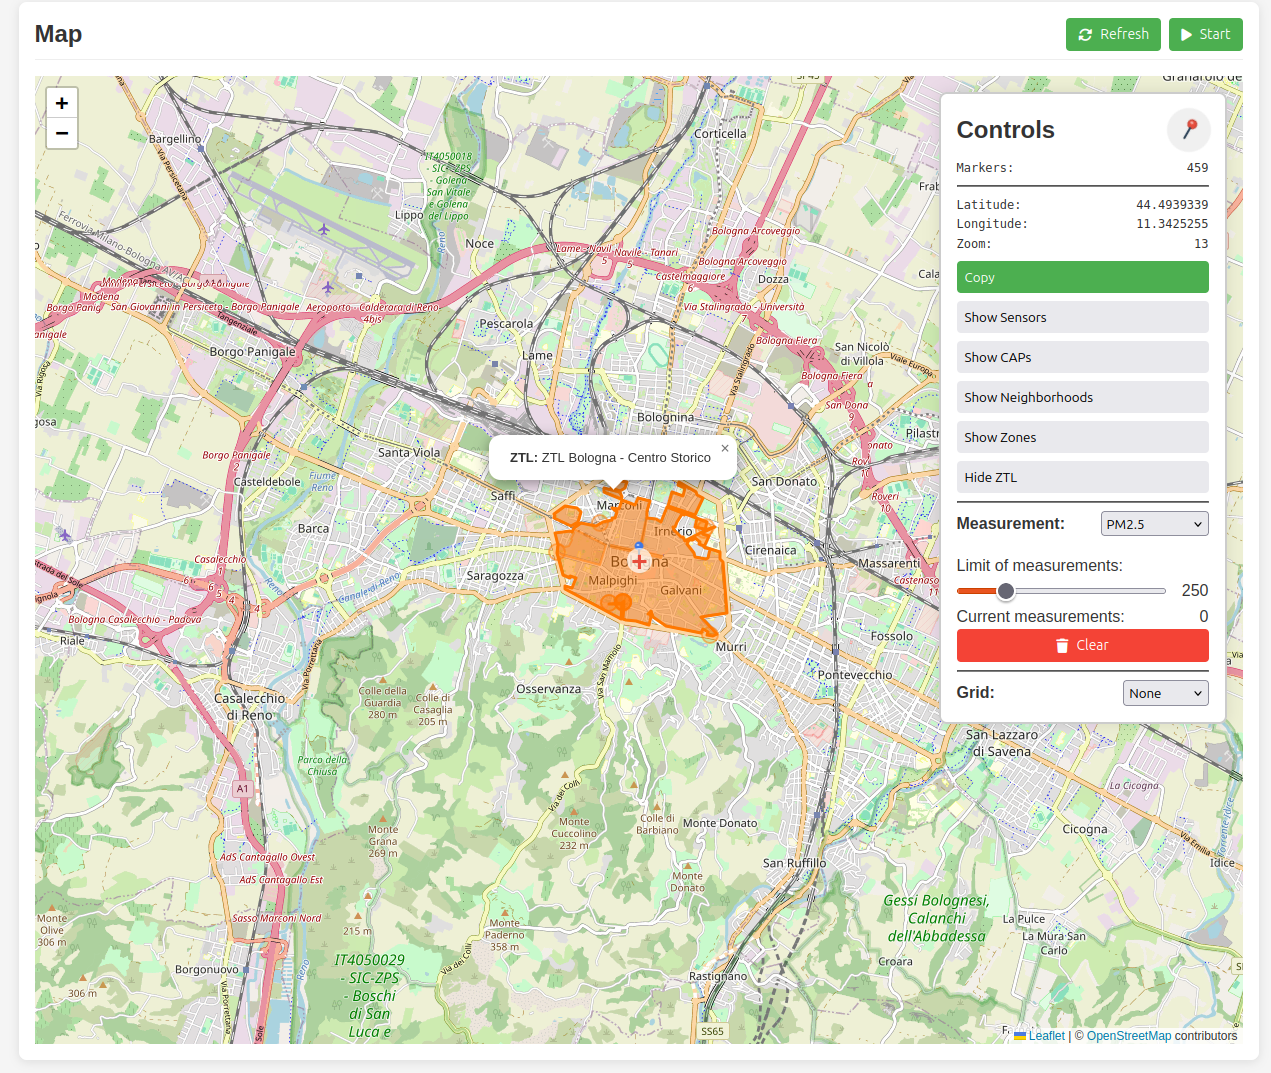
\includegraphics[width=0.95\textwidth]{dashboard/11_map_ztl_controls.png}
  \caption{Livello \acrshort{ztl}}
  \label{fig:map-layer-ztl}
\end{figure}

\newpage

\begin{figure}[H]
  \centering

  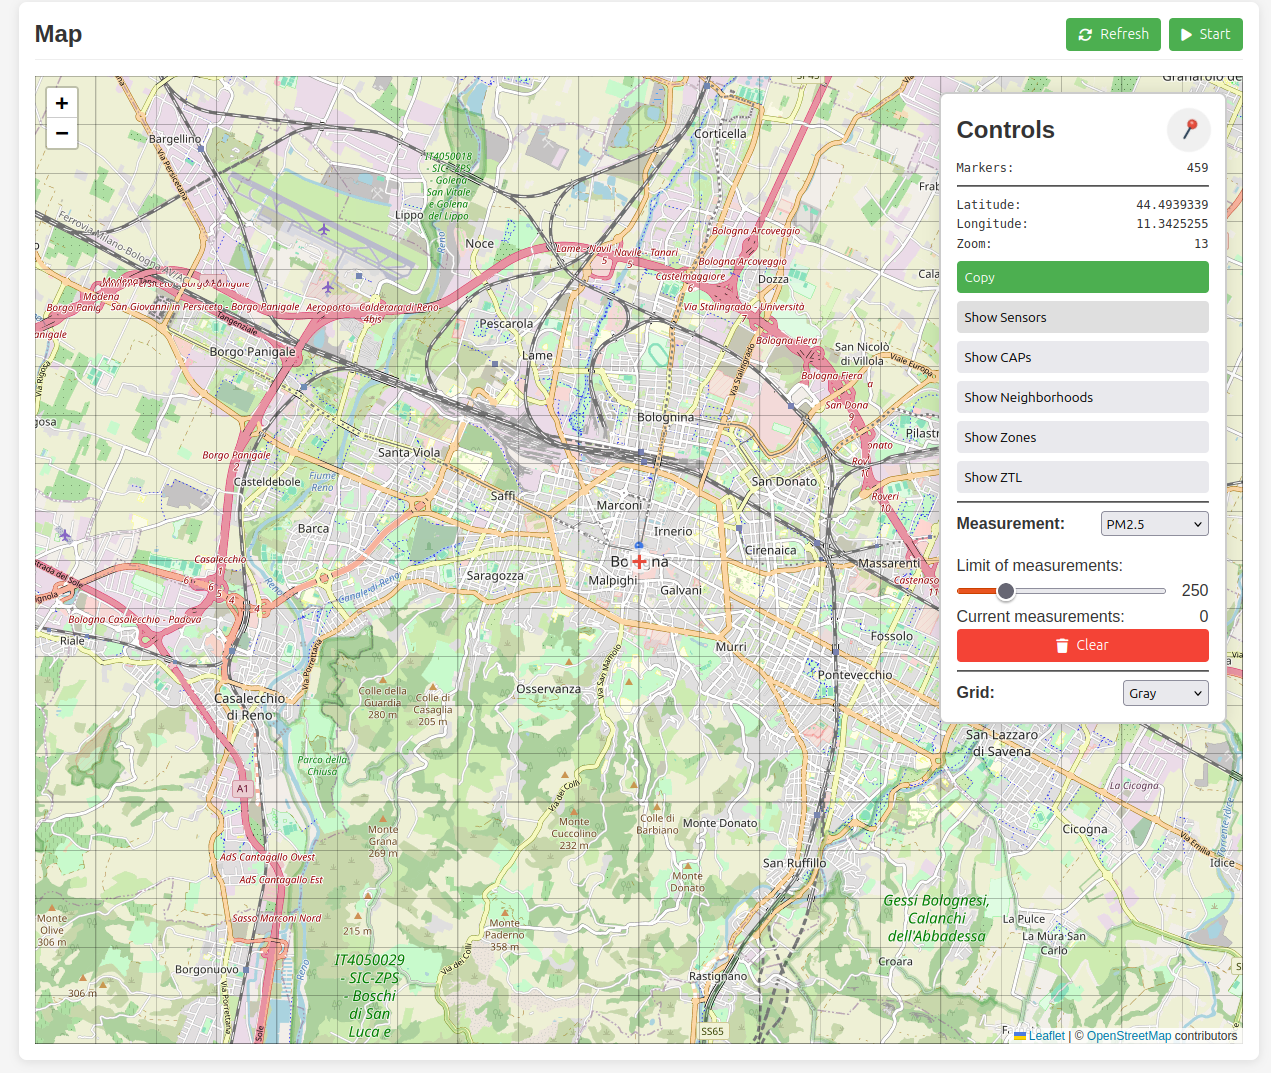
\includegraphics[width=0.95\textwidth]{dashboard/12_map_grid_gray_controls.png}
  \caption{Griglia grigia}
  \label{fig:map-grid-gray}

  \hfill

  \centering
  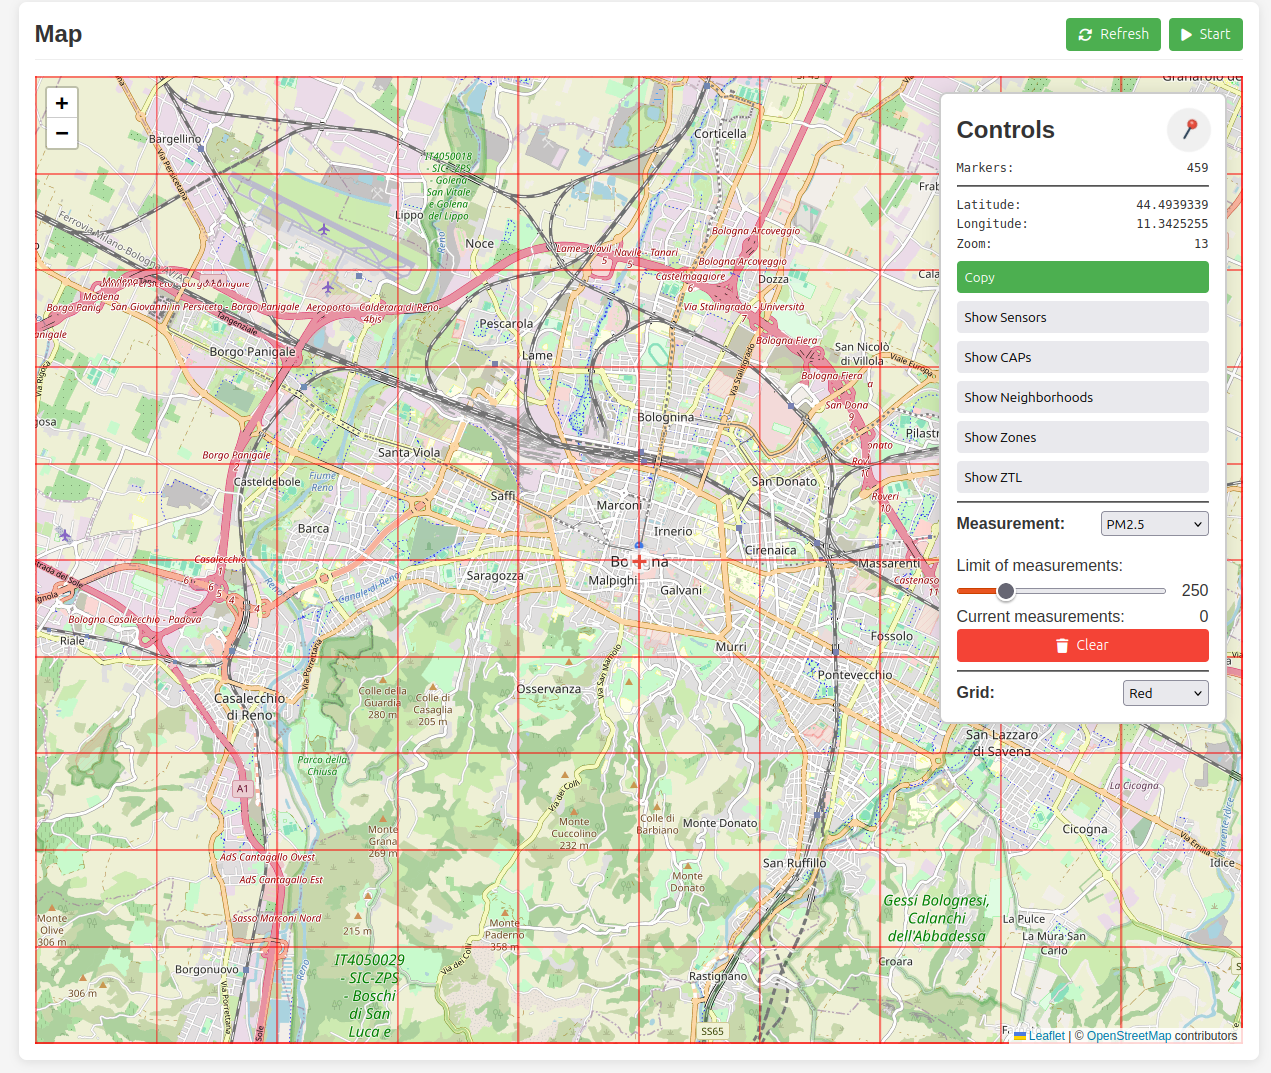
\includegraphics[width=0.95\textwidth]{dashboard/13_map_grid_red_controls.png}
  \caption{Griglia rossa}
  \label{fig:map-grid-red}
\end{figure}

\begin{figure}[H]
  \centering
  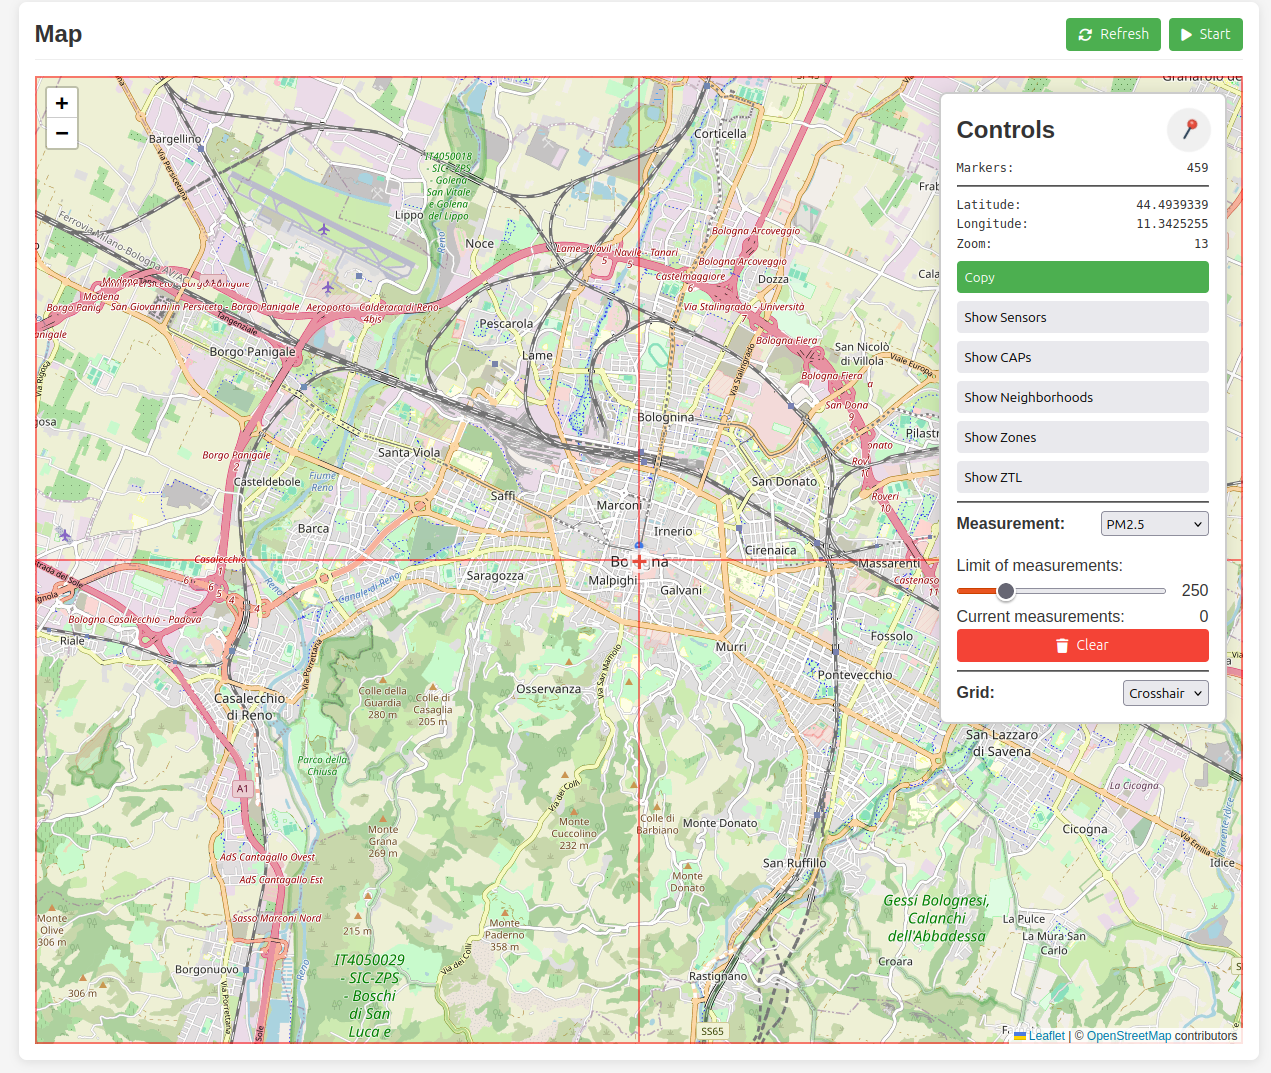
\includegraphics[width=0.95\textwidth]{dashboard/14_map_grid_crosshair_controls.png}
  \caption{Griglia crosshair}
  \label{fig:map-grid-crosshair}
\end{figure}

\newpage

\paragraph{Heatmap}

Una heatmap (mappa di calore) è una rappresentazione grafica bidimensionale di dati in cui i valori individuali,
contenuti in una matrice, sono rappresentati attraverso colori \citep{wilkinson2009grammar}.
Questa tecnica di visualizzazione permette di identificare rapidamente pattern, correlazioni e anomalie
all'interno di dataset complessi mediante l'uso di una scala cromatica che associa intensità di colore
a valori numerici \citep{cleveland1993visualizing}. Il suo utilizzo aiuta a rendere più intuitiva la distribuzione
dei dati poiché a maggior concentrazione risulta un colore più intenso, facilitandone la comprensione ed attirando
l'attenzione sui principali focolai.

Formalmente, data una matrice $M \in \mathbb{R}^{m \times n}$ dove $M_{ij}$ rappresenta il valore
nella posizione $(i,j)$, una heatmap è una funzione di mappatura $ f: M_{ij} \rightarrow C_{ij} $
dove $C_{ij}$ è il colore corrispondente al valore $M_{ij}$ secondo una scala cromatica predefinita.

La scelta della palette di colori è cruciale per l'efficacia comunicativa della heatmap.
È fondamentale utilizzare scale cromatiche che rispettino principi di accessibilità e che siano percettivamente
uniformi \citep{ware2012information}.
Tali colori sono infatti quelli forniti dall'\acrfull{eea} come indicato nella tabella~\ref{tab:air_quality};

Nelle immagini seguenti viene mostrata la heatmap relativa alle misurazioni di \acrshort{pm25}.
Partendo dalla vista default in immagine \ref{fig:app-map-pm25-controls-15},
passiamo ad una versione con zoom inferiore senza sensori \ref{fig:app-map-pm25-controls-16} e
con sensori \ref{fig:app-map-pm25-controls-17}.
Successivamente diminuiamo ulteriormente lo zoom senza sensori \ref{fig:app-map-pm25-controls-18}, per poi
riavvicinarci \ref{fig:app-map-pm25-controls-19},
visualizzarle la \acrshort{ztl} \ref{fig:app-map-pm25-controls-20} ed i quartieri\ref{fig:app-map-pm25-controls-21}.
Infine, visualizziamo una versione con concentrazioni più elevate \ref{fig:app-map-pm25-controls-22}
rispetto alle prime, essendo passato più tempo ed avendo quindi un numero maggiore di misurazioni, e le altre
misurazioni disponibili \ref{fig:app-map-pm25-controls-23}.

Come anticipato, allontanarci dal centro della mappa porterà a concentrazioni maggiori, mentre avvicinarci il contrario.
Anche il numero di misurazioni influisce sulle concentrazioni della mappa di calore, essendo direttamente correlate.
% L'utilizzo delle zone delimitate quali ZTL ed i quartieri può essere utile qualora si voglia verificare
% eventuali correlazioni fra le aree di maggiore concentrazione di inquinanti ed i confini amministrativi.

\begin{figure}[H]
  \centering
  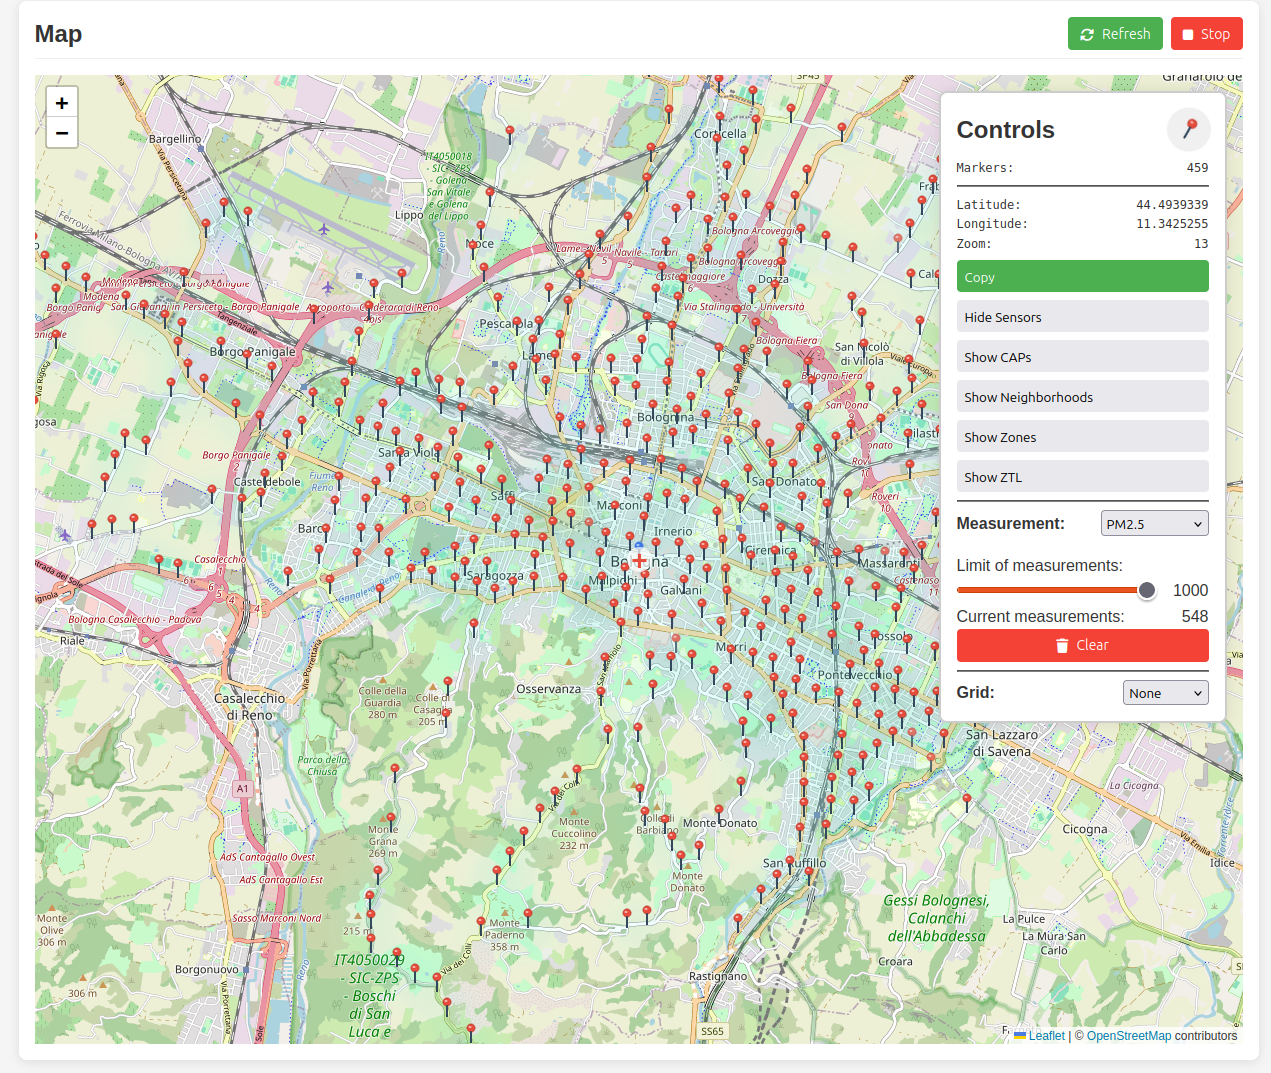
\includegraphics[width=0.95\textwidth]{dashboard/15_map_pm25_controls.png}
  \caption{Heatmap default}
  \label{fig:app-map-pm25-controls-15}

  \hfill

  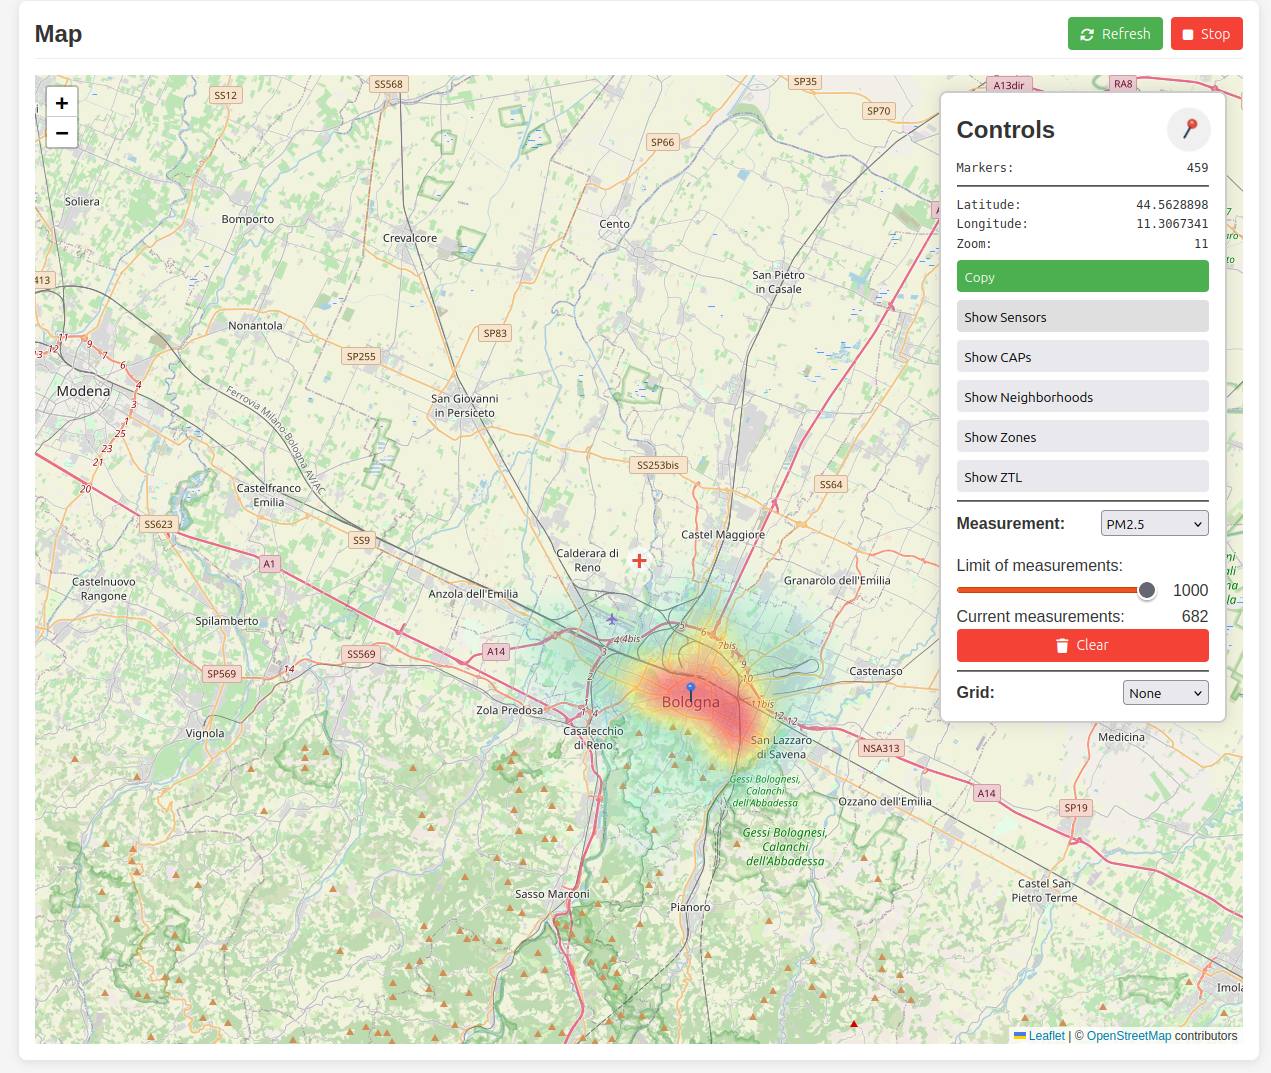
\includegraphics[width=0.95\textwidth]{dashboard/16_map_pm25_controls.png}
  \caption{Heatmap zoom 11 senza sensori}
  \label{fig:app-map-pm25-controls-16}
\end{figure}

\begin{figure}[H]
  \centering
  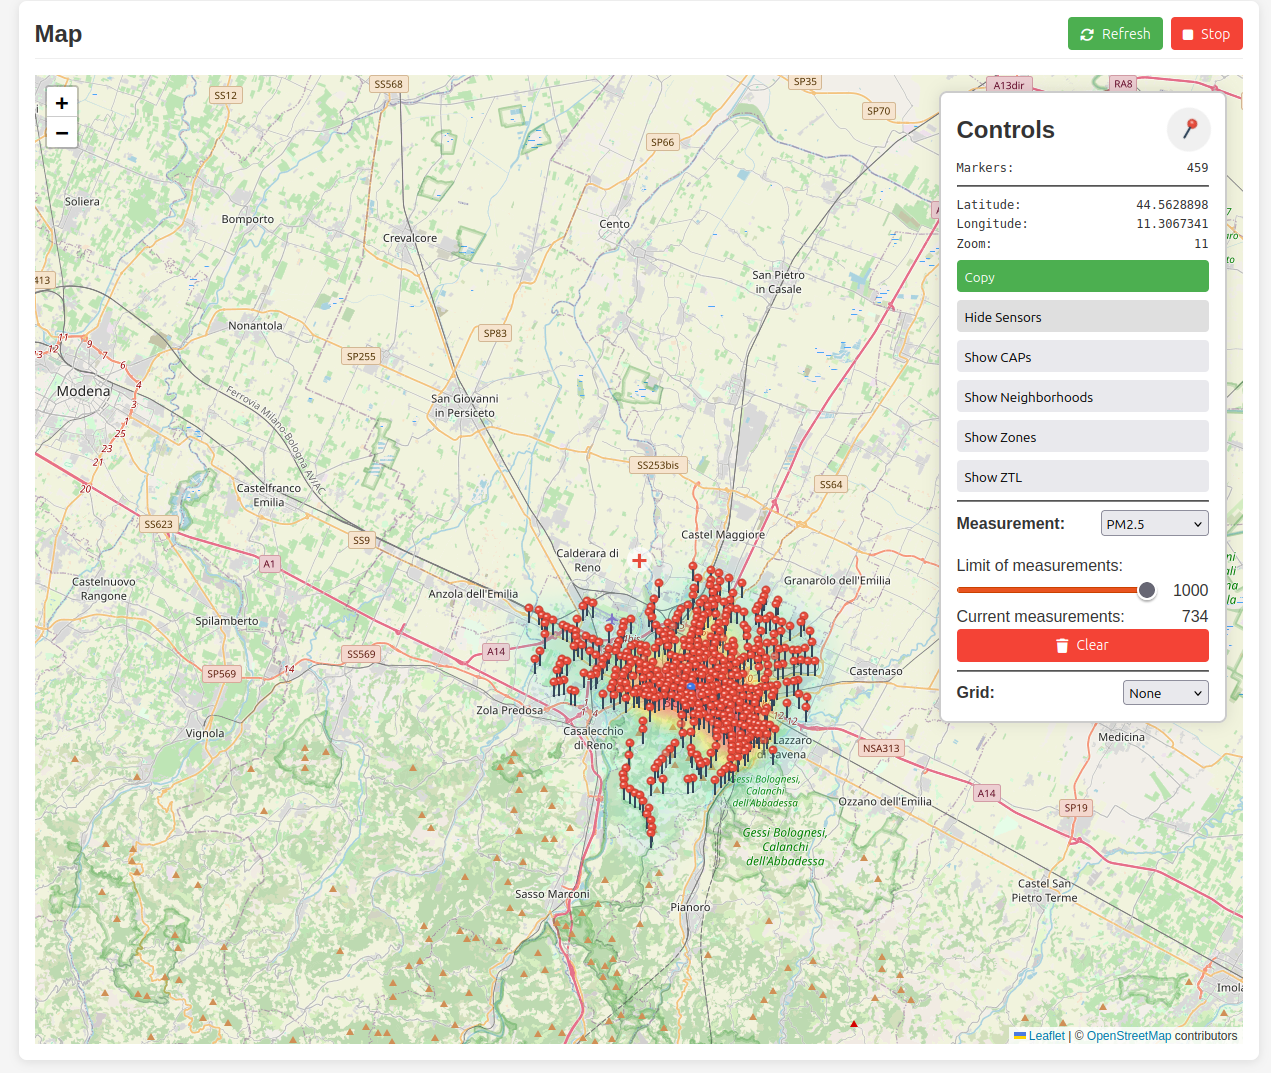
\includegraphics[width=0.95\textwidth]{dashboard/17_map_pm25_controls.png}
  \caption{Heatmap zoom 11 con sensori}
  \label{fig:app-map-pm25-controls-17}

  \hfill

  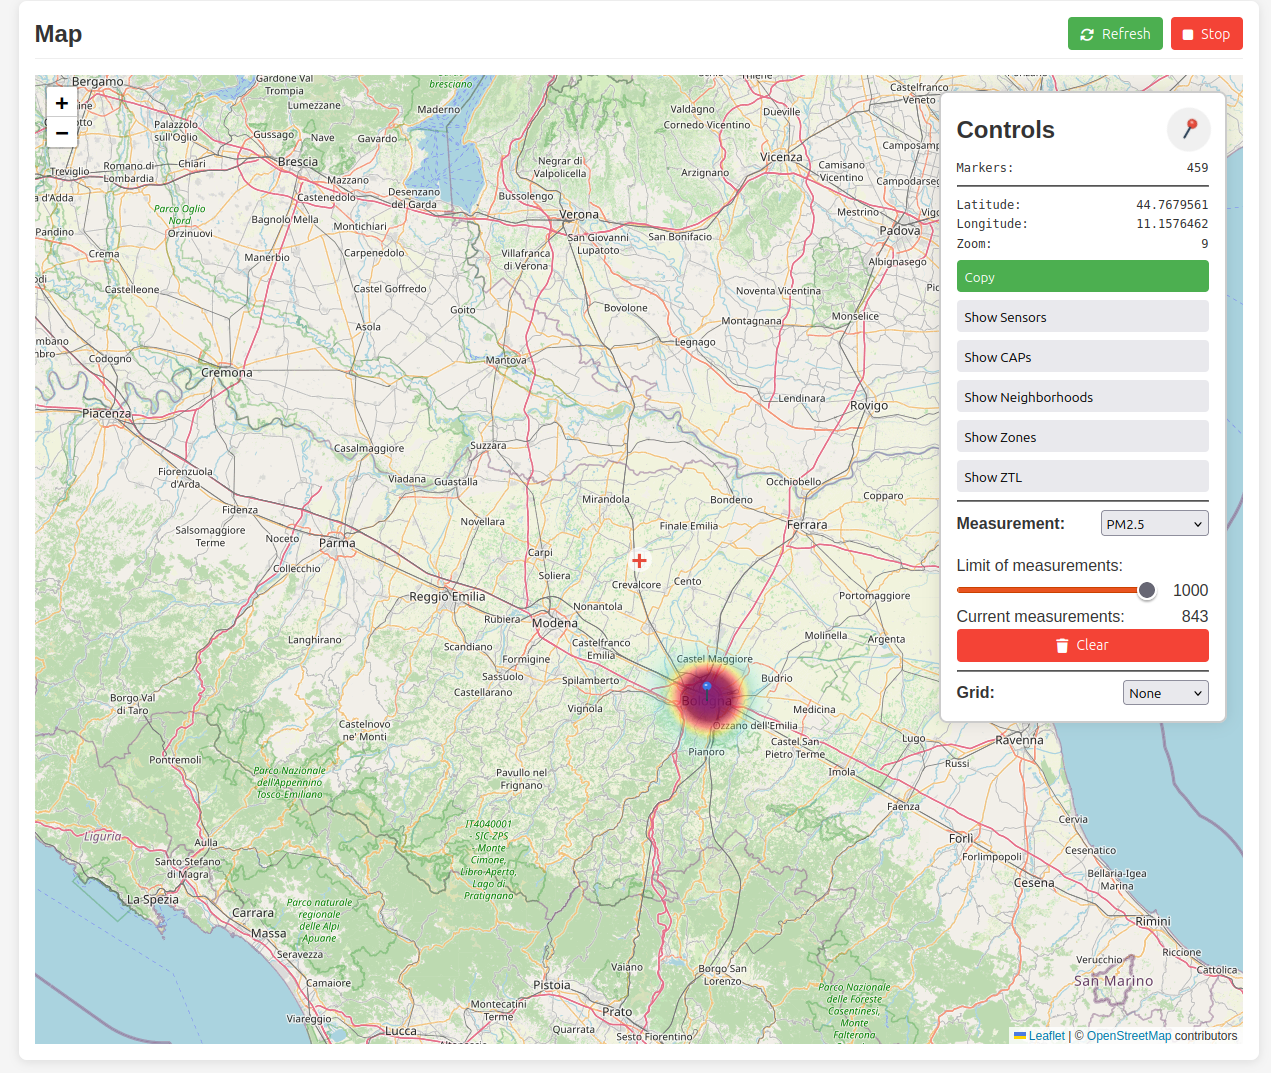
\includegraphics[width=0.95\textwidth]{dashboard/18_map_pm25_controls.png}
  \caption{Heatmap zoom 9 senza sensori}
  \label{fig:app-map-pm25-controls-18}
\end{figure}

\begin{figure}[H]
  \centering
  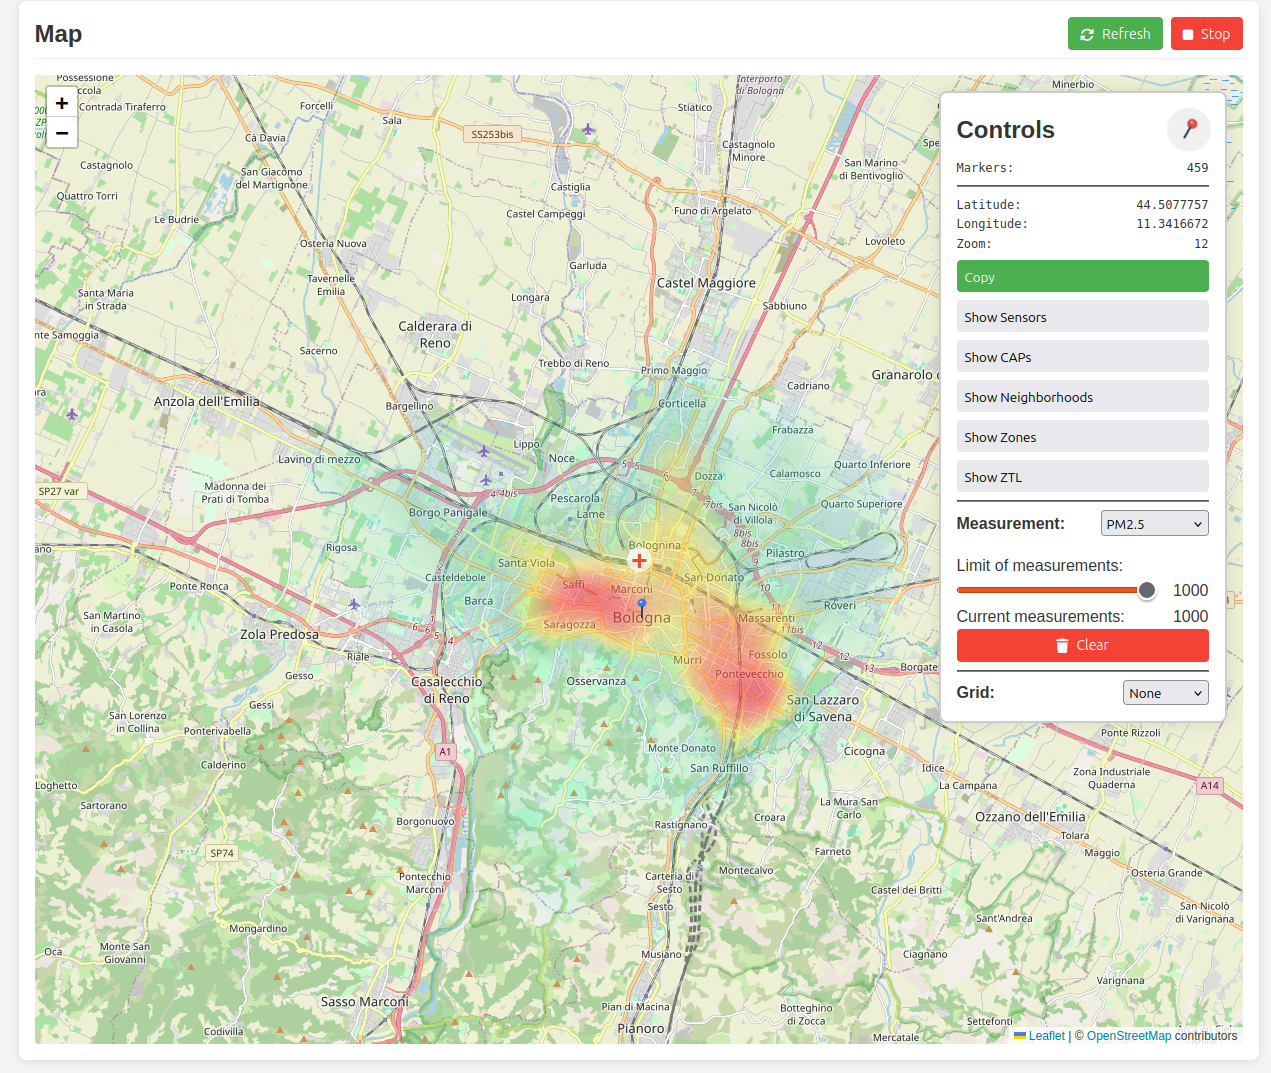
\includegraphics[width=0.95\textwidth]{dashboard/19_map_pm25_controls.png}
  \caption{Heatmap zoom 12 senza sensori}
  \label{fig:app-map-pm25-controls-19}

  \hfill

  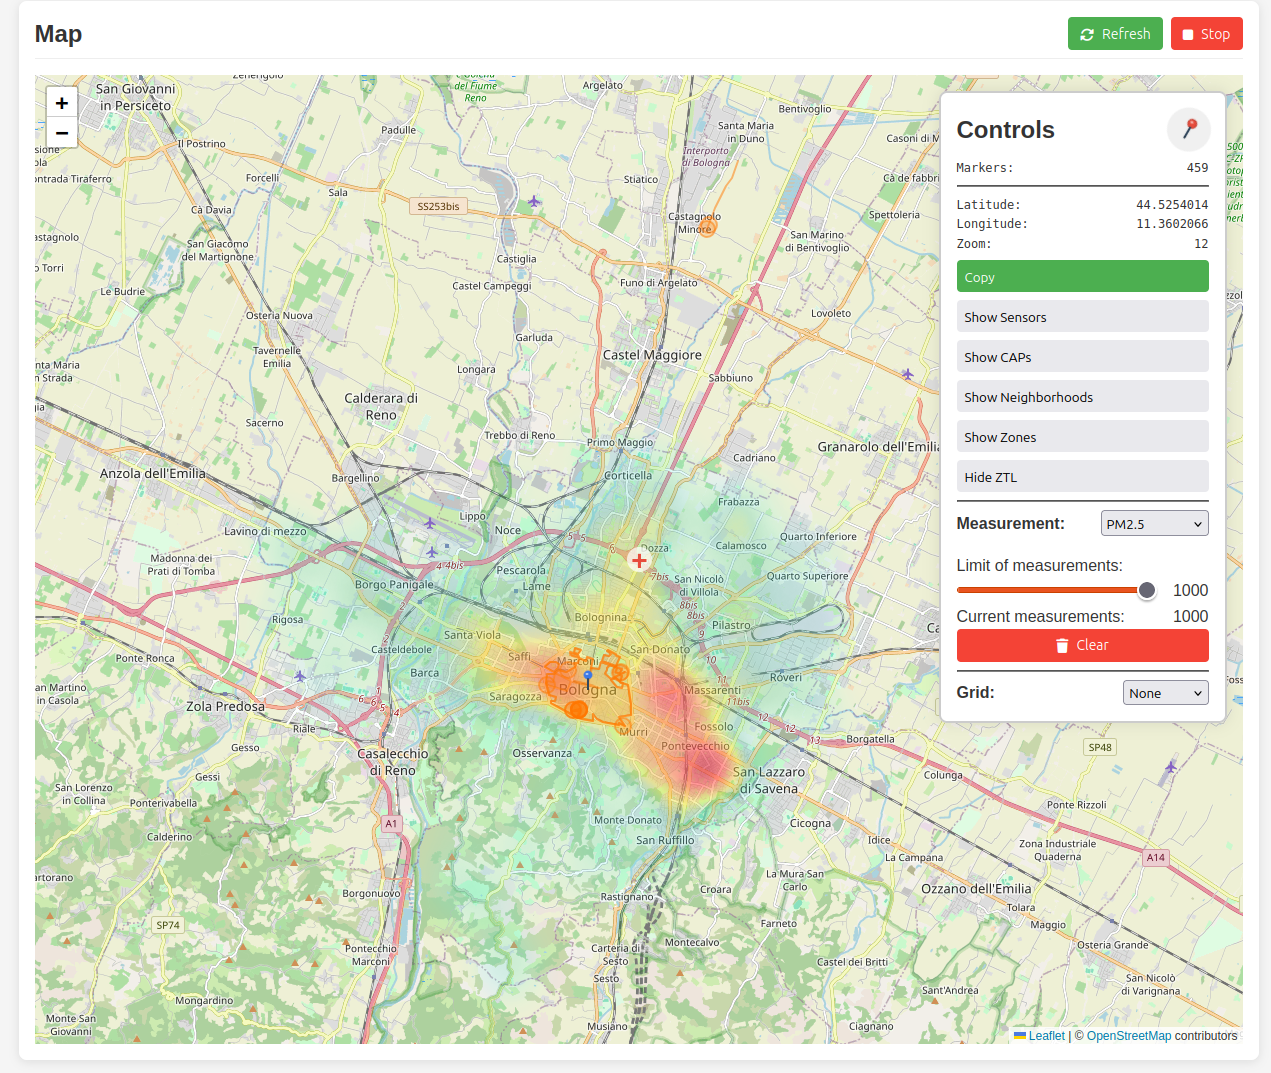
\includegraphics[width=0.95\textwidth]{dashboard/20_map_pm25_controls.png}
  \caption{Heatmap zoom 12 senza sensori con \acrshort{ztl}}
  \label{fig:app-map-pm25-controls-20}
\end{figure}

\begin{figure}[H]
  \centering
  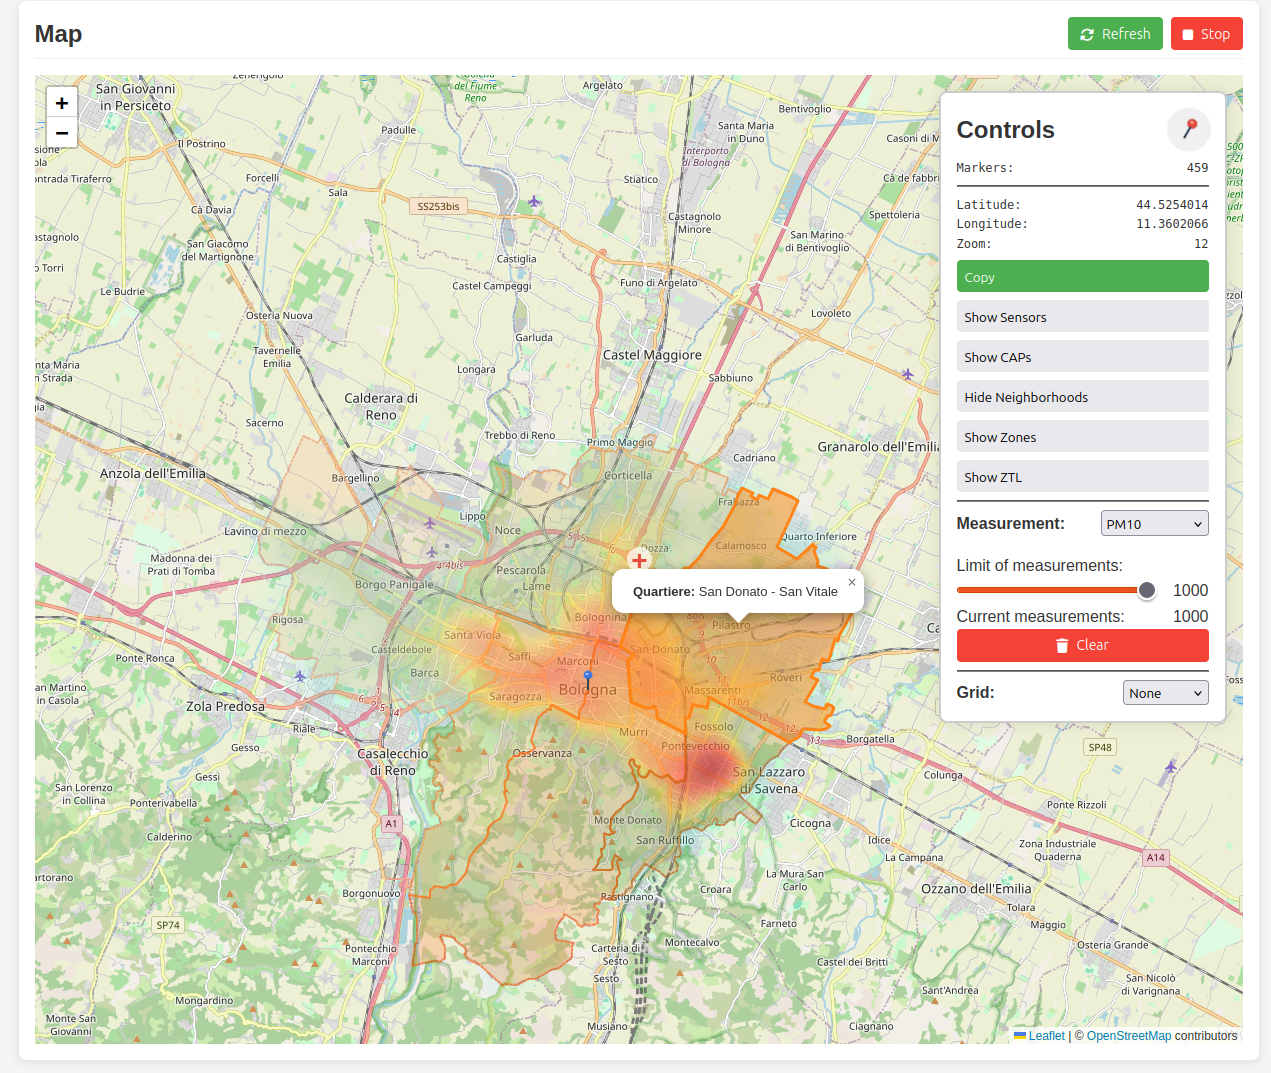
\includegraphics[width=0.95\textwidth]{dashboard/21_map_pm25_controls.png}
  \caption{Heatmap zoom 12 senza sensori con quartieri}
  \label{fig:app-map-pm25-controls-21}

  \hfill

  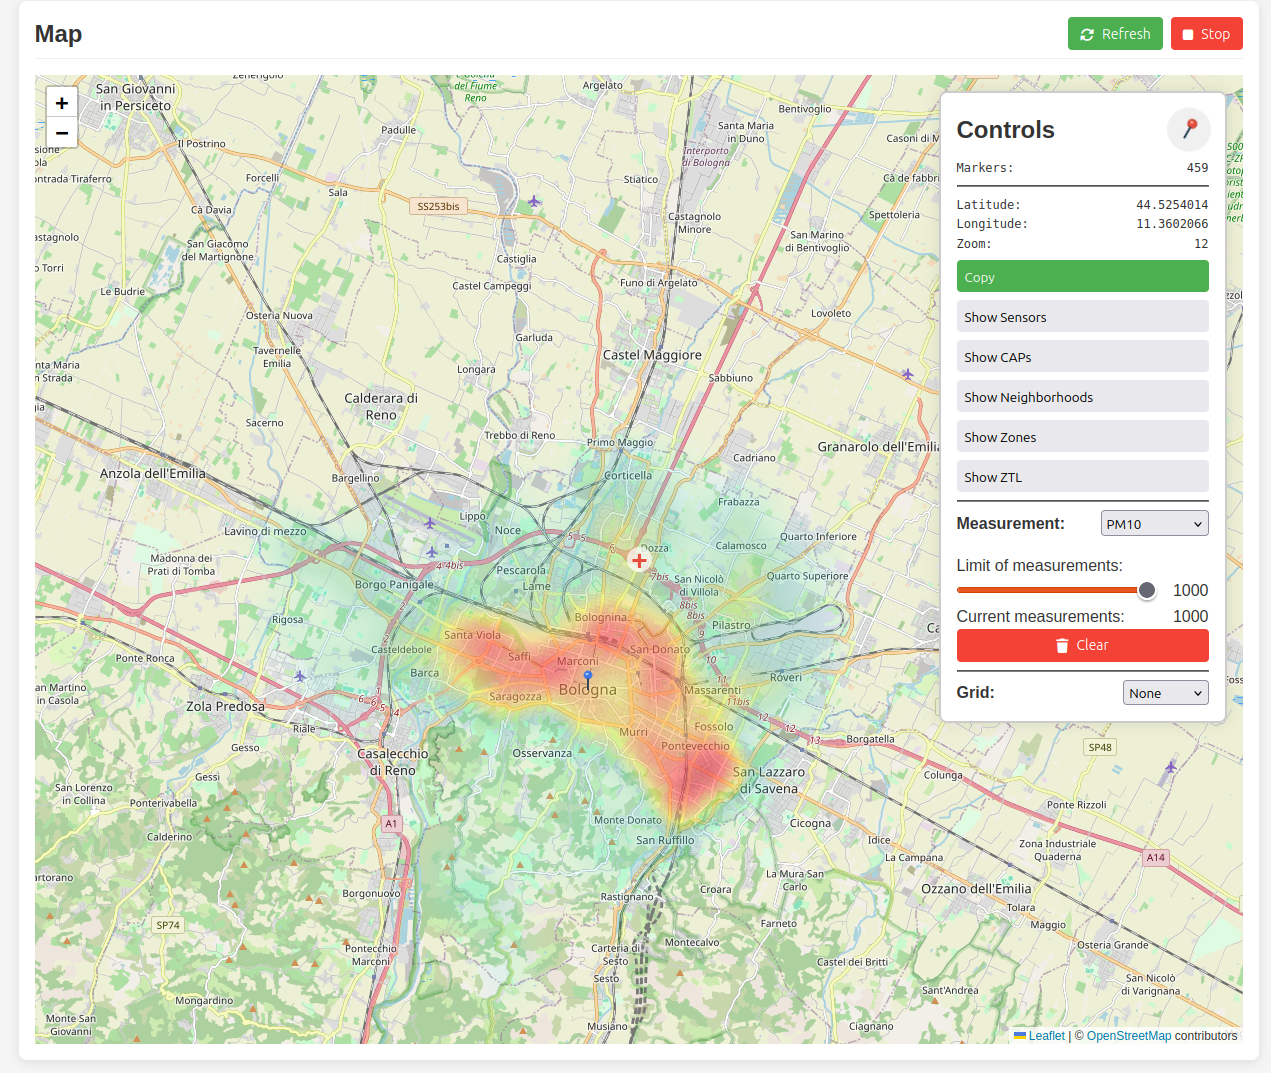
\includegraphics[width=0.95\textwidth]{dashboard/22_map_pm25_controls.png}
  \caption{Heatmap zoom 12 senza sensori, concentrazione maggiore}
  \label{fig:app-map-pm25-controls-22}
\end{figure}

\begin{figure}[H]
  \centering
  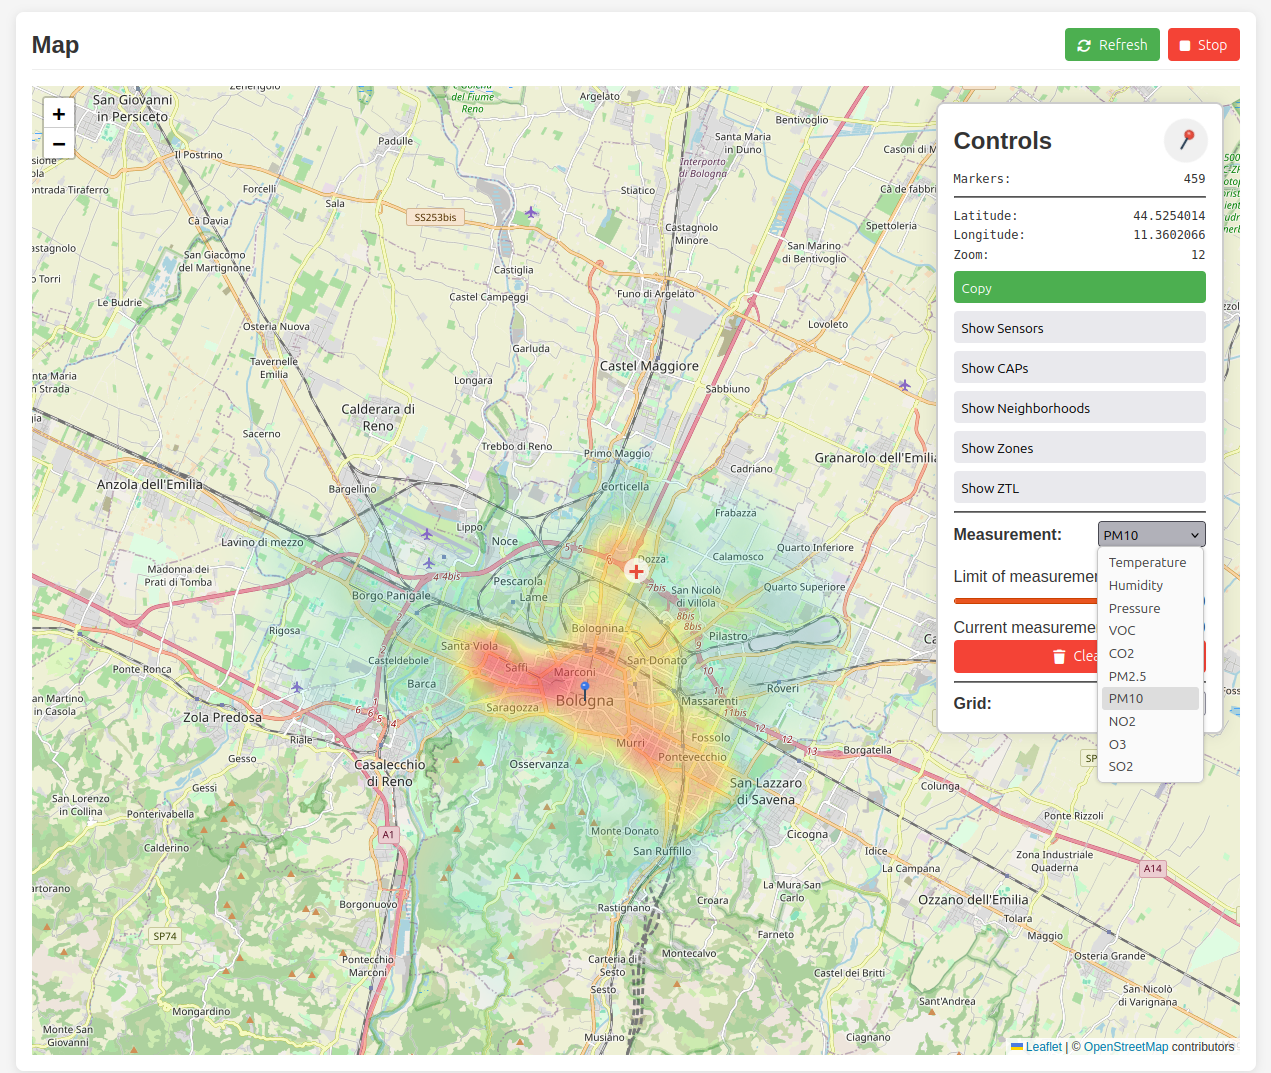
\includegraphics[width=0.95\textwidth]{dashboard/23_map_pm25_controls.png}
  \caption{Heatmap zoom 12 senza sensori, apertura lista misurazioni disponibili}
  \label{fig:app-map-pm25-controls-23}
\end{figure}

\newpage

\paragraph{Ultime misurazioni}

La tabella delle misurazioni illustrata nella figura~\ref{fig:app-tab-last-measurements} offre una visualizzazione
organizzata delle ultime 50 rilevazioni acquisite dal sistema. Ogni misurazione viene presentata su una riga separata,
contenente informazioni essenziali come l'identificativo del sensore, il momento preciso dell'acquisizione e tutti
i parametri rilevati con le corrispondenti unità di misura.
L'interfaccia è progettata per facilitare la navigazione: selezionando una qualsiasi riga della tabella,
l'utente viene automaticamente reindirizzato alla vista mappa centrata sul sensore responsabile
di quella specifica rilevazione. Questa funzionalità permette di collegare rapidamente i dati numerici alla
loro posizione geografica, offrendo una comprensione più completa delle informazioni raccolte.
La struttura tabulare garantisce una consultazione rapida e ordinata dei dati più recenti,
mantenendo sempre visibili le informazioni più aggiornate del sistema di monitoraggio.

\begin{figure}[H]
  \centering
  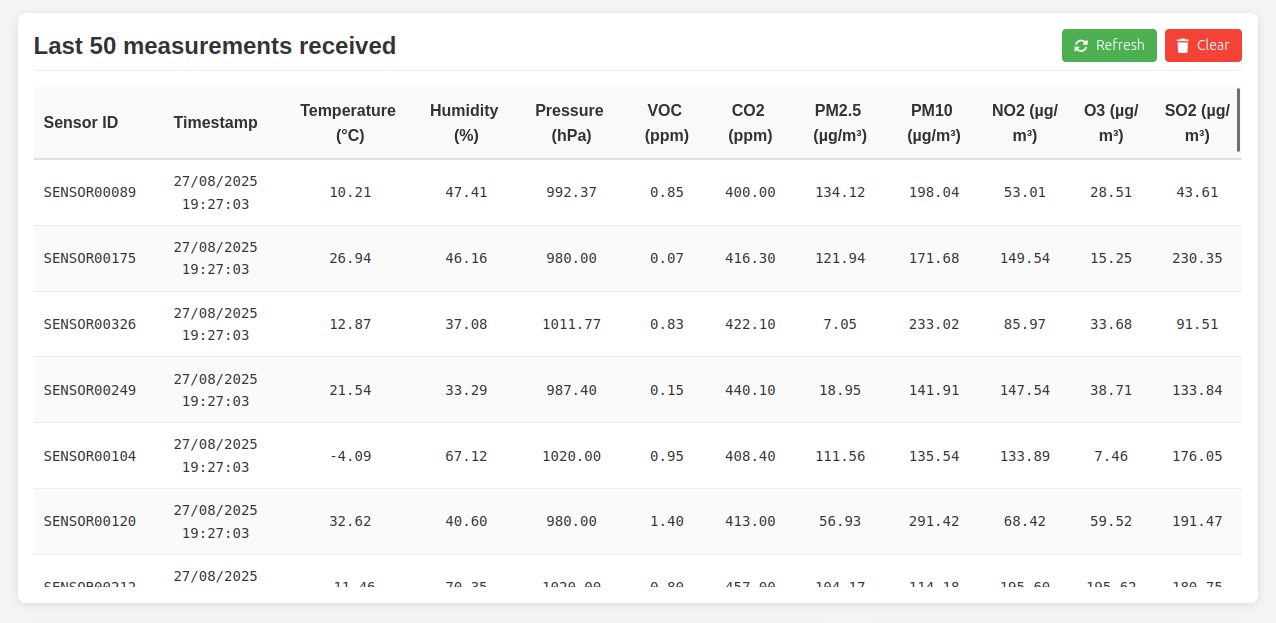
\includegraphics[width=\textwidth]{dashboard/24_table_last_measurements.png}
  \caption{Tabella ultime misurazioni}
  \label{fig:app-tab-last-measurements}
\end{figure}

\newpage

\paragraph{Statistiche}

La tabella delle statistiche riportata nell'immagine~\ref{fig:app-tab-statistics} fornisce un'analisi completa
dei dati per ogni tipologia di misurazione ambientale raccolta dal sistema. Il processo di elaborazione calcola
automaticamente gli indicatori statistici fondamentali: vengono determinati valore medio e mediana
per identificare la tendenza centrale, mentre i valori minimo e massimo evidenziano gli estremi registrati.
Il range di variazione, ottenuto dalla differenza tra questi due estremi, quantifica l'ampiezza
delle oscillazioni rilevate.
Oltre agli indicatori numerici, il sistema integra una valutazione qualitativa dell'aria specifica
per ciascun tipo di inquinante monitorato.
Questa analisi applica criteri di classificazione standardizzati riportati nella tabella~\ref{tab:air_quality},
i quali traducono i valori numerici in categorie comprensibili, accompagnate da un sistema di colori intuitivo
che permette di identificare immediatamente il livello di qualità raggiunto.
L'approccio combinato tra dati statistici e valutazione qualitativa offre agli utenti sia una comprensione
tecnica dettagliata che un'interpretazione immediata dello stato ambientale monitorato.

\begin{figure}[H]
  \centering
  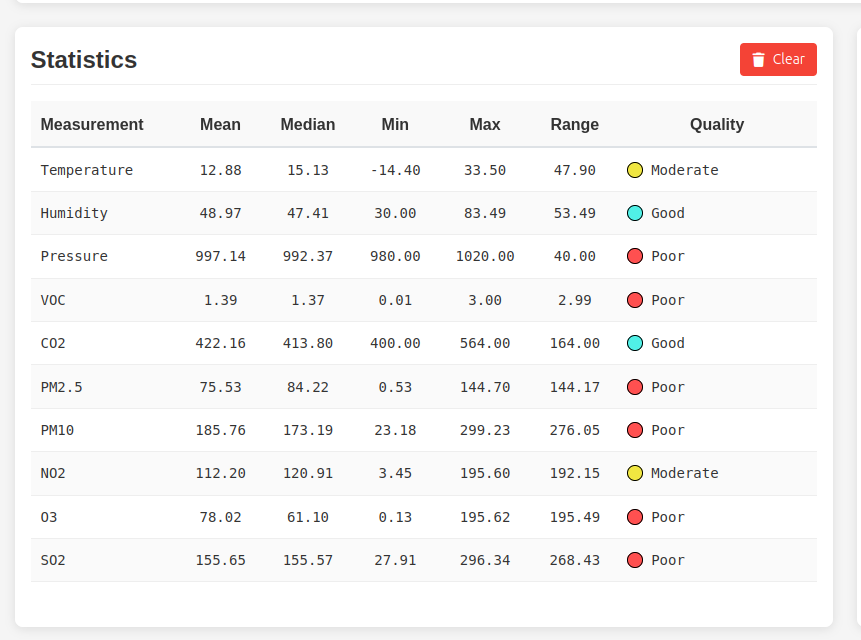
\includegraphics[width=0.9\textwidth]{dashboard/25_table_statistics.png}
  \caption{Tabella statistiche}
  \label{fig:app-tab-statistics}
\end{figure}

\newpage

\paragraph{Log di sistema}

L'applicazione mantiene un registro completo delle attività utente attraverso una tabella di log che documenta tutte
le interazioni, sia quelle effettuate tramite interfaccia grafica che attraverso chiamate \acrshort{api}, come si
può vedere nell'immagine~\ref{fig:app-tab-system-log}.
Il sistema traccia diversi tipi di eventi: l'arrivo di nuove misurazioni dai sensori, i clic sui dispositivi
nell'interfaccia, le operazioni di registrazione dei sensori e l'attivazione o disattivazione della ricezione dati.
Per ottimizzare la visualizzazione, il log raggruppa automaticamente gli eventi identici che si verificano
nel medesimo secondo, mostrando il numero di occorrenze (in grigio) accanto alla voce principale.
Questa funzionalità evita la duplicazione di informazioni e mantiene il registro più leggibile.
Il sistema limita la visualizzazione a un massimo di 25 righe per garantire prestazioni ottimali e una consultazione
agevole. Quando questo limite viene raggiunto, le voci più recenti sostituiscono automaticamente quelle più datate,
assicurando che il log mostri sempre le attività più attuali del sistema.

\begin{figure}[H]
  \centering
  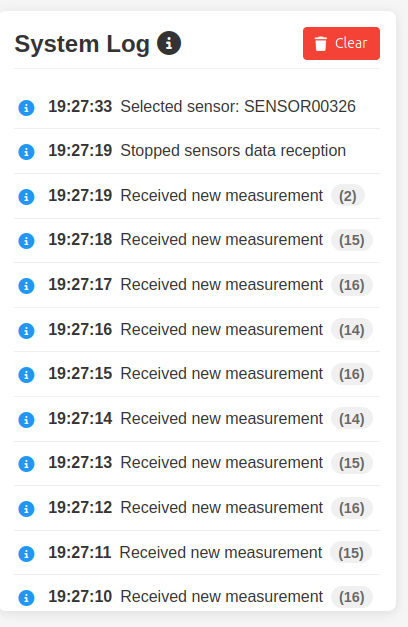
\includegraphics[width=0.45\textwidth]{dashboard/26_table_system_log.png}
  \caption{Tabella log di sistema}
  \label{fig:app-tab-system-log}
\end{figure}

\newpage

\paragraph{Tabella dei sensori registrati}

La parte finale della pagina principale riporta la tabella dei sensori registrati.

Questa tabella è formata da diverse colonne, quali l'id del sensore, latitudine, longitudine, stato,
distanza dal centro della mappa, data ultima misurazione registrata e relativo tempo trascorso da essa.

\begin{figure}[H]
  \centering
  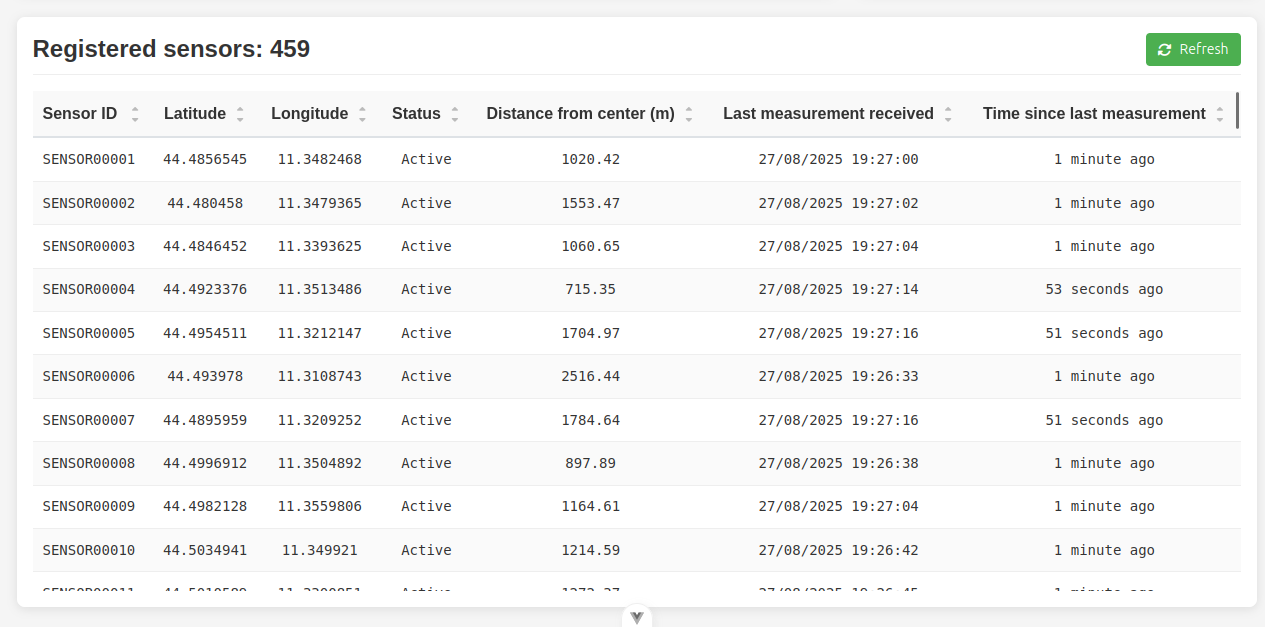
\includegraphics[width=\textwidth]{dashboard/27_table_registered_sensors.png}
  \caption{Tabella sensori registrati}
  \label{fig:app-tab-registered-sensors}
\end{figure}

Nella prima immagine~\ref{fig:app-tab-registered-sensors} abbiamo i sensori ordinati per id crescente (default),
mentre nella seconda~\ref{fig:app-tab-registered-sensors-distance-sort-asc} e
terza immagine~\ref{fig:app-tab-registered-sensors-distance-sort-desc} si ha la tabella ordinata rispetto
la distanza dal centro della mappa relativamente in ordine crescente (dal sensore più prossimo al più remoto) e
decrescente (dal sensore più lontano al più vicino).
Anche qui, cliccando sulla riga dedicata, la pagina scorre verso la mappa centrata sul sensore indicato.

\begin{figure}[H]
  \centering
  \begin{subfigure}{\textwidth}
    \centering
    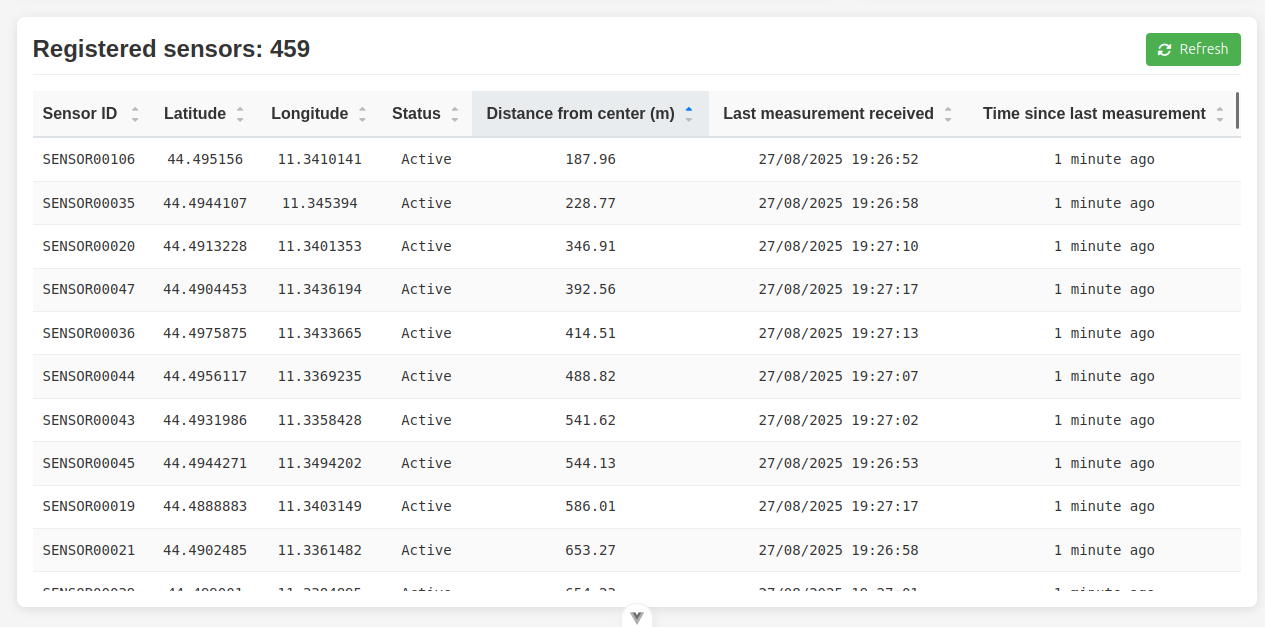
\includegraphics[width=\textwidth]{dashboard/28_table_registered_sensors_distance_sort_asc.png}
    \caption{Tabella sensori registrati, ordinati per "distanza dal centro" crescente}
    \label{fig:app-tab-registered-sensors-distance-sort-asc}
  \end{subfigure}

  \hfill
  \begin{subfigure}{\textwidth}
    \centering
    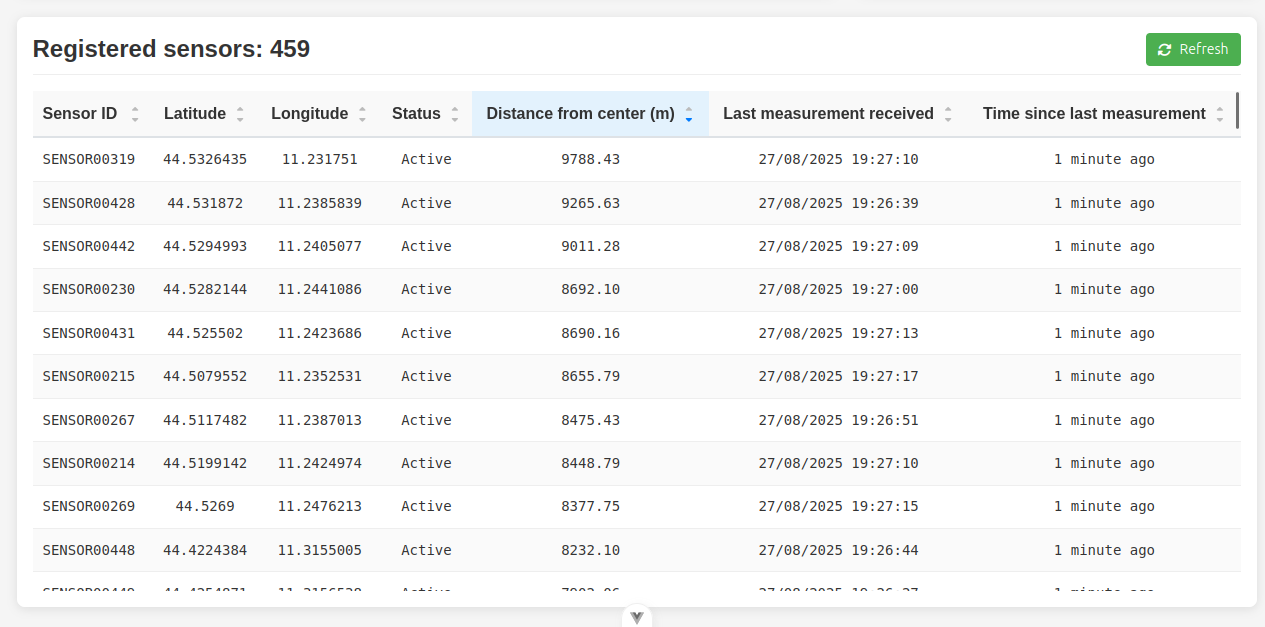
\includegraphics[width=\textwidth]{dashboard/29_table_registered_sensors_distance_sort_desc.png}
    \caption{Tabella sensori registrati, ordinati per "distanza dal centro" decrescente}
    \label{fig:app-tab-registered-sensors-distance-sort-desc}
  \end{subfigure}
\end{figure}

Il calcolo per tale distanza è realizzato attraverso la formula di Haversine \cite{haversine_formula},
ovvero una funzione usata per calcolare la distanza ortodromica (linea retta sulla superficie terrestre) tra due punti.
Essendo i sensori dotati di coordinate spaziali quali latitudine e longitudine, come il centro della mappa,
la formula è risultata l'ideale per calcolarne la distanza.

\paragraph{Formula di Haversine}

Di seguito la formula in termini matematici~\ref{lst:haversine-formula-math},
con relativa legenda~\ref{lst:haversine-formula-math-legend}, e la versione
di codice Javascript~\ref{lst:haversine-formula-code} realmente utilizzata dall'applicazione.

\begin{figure}[h]
  \begin{align}
    a & = \sin^2\left(\frac{\Delta\varphi}{2}\right) + \cos\varphi_1 \cdot \cos\varphi_2 \cdot \sin^2\left(\frac{\Delta\lambda}{2}\right) \\
    c & = 2 \cdot \text{atan2}\left(\sqrt{a}, \sqrt{1-a}\right)                                                                           \\
    d & = R \cdot c
  \end{align}
  \caption{Formula matematica di Haversine}
  \label{lst:haversine-formula-math}
\end{figure}

\begin{tabular}{ll}
  \textbf{Simbolo}       & \textbf{Significato}                                \\
  \hline
  $\varphi$              & latitudine (in radianti)                            \\
  $\varphi_1, \varphi_2$ & latitudine del punto 1 e punto 2                    \\
  $\Delta\varphi$        & differenza di latitudine ($\varphi_2 - \varphi_1$)  \\
  $\lambda$              & longitudine (in radianti)                           \\
  $\lambda_1, \lambda_2$ & longitudine del punto 1 e punto 2                   \\
  $\Delta\lambda$        & differenza di longitudine ($\lambda_2 - \lambda_1$) \\
  $R$                    & raggio terrestre medio ($\sim 6371$ km)          \\
  $d$                    & distanza tra i punti (in metri o km)                \\
  $c$                    & distanza angolare (in radianti)                     \\
  $a$                    & termine intermedio                                  \\
  \label{lst:haversine-formula-math-legend}
\end{tabular}

\begin{lstlisting}[caption={Formual di Haversine in codice Javascript}, label=lst:haversine-formula-code]
  // Function to calculate the distance between two geographic points (Haversine formula)
  calculateDistance(lat1, lon1, lat2, lon2) {
    const R = 6371000; // Earth radius in meters
    const dLat = ((lat2 - lat1) * Math.PI) / 180;
    const dLon = ((lon2 - lon1) * Math.PI) / 180;
    const a =
      Math.sin(dLat / 2) * Math.sin(dLat / 2) +
      Math.cos((lat1 * Math.PI) / 180) *
      Math.cos((lat2 * Math.PI) / 180) *
      Math.sin(dLon / 2) *
      Math.sin(dLon / 2);
    const c = 2 * Math.atan2(Math.sqrt(a), Math.sqrt(1 - a));
    return R * c;
  }
\end{lstlisting}

\section{Database service}

In questa sezione verrà descritto il servizio di database, per il quale è stato scelto il database non relazione
Mongodb.

Il database MongoDB è stato progettato per gestire efficacemente i dati di sistemi analoghi a quelli del progetto.
L'architettura del database si basa su due collezioni principali per mantenere le informazioni relative ai
sensori e alle relative misurazioni simulate della qualità dell'aria.

La prima collezione, denominata \texttt{sensors}, è dedicata alla gestione anagrafica dei dispositivi di rilevamento.
Ogni sensore viene identificato in modo univoco attraverso un codice alfanumerico generato automaticamente e comprende
informazioni essenziali come il nome del dispositivo, la sua posizione geografica espressa in formato GeoJSON
con coordinate longitude-latitude, l'indirizzo \acrshort{ip} assegnato e lo stato di attività.
Il sistema mantiene inoltre traccia dell'ultimo contatto con ciascun sensore per monitorare la disponibilità
della rete di rilevamento.

La seconda collezione, \texttt{measurements}, costituisce il cuore del sistema di archiviazione dati,
conservando tutte le misurazioni ambientali acquisite nel tempo. Ogni rilevazione comprende un riferimento al sensore
di origine, il timestamp preciso dell'acquisizione e un set completo di parametri ambientali: temperatura,
umidità relativa, pressione atmosferica, concentrazione di composti organici volatili, livelli di \acrshort{co2},
particolato fine \acrshort{pm25} e \acrshort{pm10}, e concentrazioni di inquinanti gassosi come \acrshort{no2},
\acrshort{o3} e \acrshort{so2}.

Il sistema di inizializzazione automatizza completamente la configurazione del database.
Durante l'avvio, vengono create le collezioni con validatori di schema che garantiscono l'integrità
strutturale dei dati, vengono popolati i sensori utilizzando coordinate geografiche caricate
da file \acrshort{json} esterno ottenuto dal sistema citato in~\ref{subsection:sensor-distribution}, e vengono
configurati gli indici necessari per ottimizzare le prestazioni di ricerca. L'indicizzazione include chiavi univoche
per gli identificatori dei sensori, indici geospaziali per le query di prossimità geografica, e indici composti
per ottimizzare l'accesso cronologico alle misurazioni.

Nelle seguenti liste viene indicato il codice Javascript atto alla creazione delle collezioni
\texttt{sensors}~\ref{lst:mongodb-sensors}, \texttt{measurements}~\ref{lst:mongodb-measurements} e relativi
indici~\ref{lst:mongodb-indexes}.

\begin{lstlisting}[caption={Generazione collezione \texttt{sensors} MongoDB}, label=lst:mongodb-sensors]
// Sensors collection
db.createCollection("sensors", {
  validator: {
    $jsonSchema: {
      bsonType: "object",
      required: ["sensor_id", "name", "location", "ip"],
      properties: {
        sensor_id: {
          bsonType: "string",
          description: "Unique identifier for the sensor",
        },
        name: {
          bsonType: "string",
          description: "Name of the sensor",
        },
        location: {
          bsonType: "object",
          required: ["type", "coordinates"],
          properties: {
            type: {
              bsonType: "string",
              enum: ["Point"],
              description: "GeoJSON type",
            },
            coordinates: {
              bsonType: "array",
              minItems: 2,
              maxItems: 2,
              items: {
                bsonType: "double",
                description: "[longitude, latitude]",
              },
            },
          },
        },
        ip: {
          bsonType: "string",
          description: "IP address of the sensor",
        },
        active: {
          bsonType: "bool",
          description: "Whether the sensor is currently active",
        },
        last_seen: {
          bsonType: "date",
          description: "Last time the sensor reported data",
        },
      },
    },
  },
});
\end{lstlisting}

\begin{lstlisting}[caption={Generazione collezione \texttt{measurements} MongoDB}, label=lst:mongodb-measurements]
// Measurements collection
db.createCollection("measurements", {
  validator: {
    $jsonSchema: {
      bsonType: "object",
      required: [
        "sensor_id",
        "timestamp",
        "temperature",
        "humidity",
        "pressure",
        "voc",
        "co2",
        "pm25",
        "pm10",
        "no2",
        "o3",
        "so2",
      ],
      properties: {
        sensor_id: {
          bsonType: "string",
          description: "Reference to the sensor",
        },
        timestamp: {
          bsonType: "date",
          description: "Time of measurement",
        },
        temperature: {
          bsonType: ["double", "int"],
          description: "Temperature in Celsius",
        },
        humidity: {
          bsonType: ["double", "int"],
          description: "Relative humidity percentage",
        },
        pressure: {
          bsonType: ["double", "int"],
          description: "Atmospheric pressure in hPa",
        },
        voc: {
          bsonType: ["double", "int"],
          description: "Volatile Organic Compounds in ppb",
        },
        co2: {
          bsonType: ["double", "int"],
          description: "CO2 concentration in ppm",
        },
        pm25: {
          bsonType: ["double", "int"],
          description: "PM2.5 concentration in micrograms/m^3",
        },
        pm10: {
          bsonType: ["double", "int"],
          description: "PM10 concentration in micrograms/m^3",
        },
        no2: {
          bsonType: ["double", "int"],
          description: "NO2 concentration in micrograms/m^3",
        },
        o3: {
          bsonType: ["double", "int"],
          description: "O3 concentration in micrograms/m^3",
        },
        so2: {
          bsonType: ["double", "int"],
          description: "SO2 concentration in micrograms/m^3",
        },
      },
    },
  },
});
\end{lstlisting}

\begin{lstlisting}[caption={Generazione indici MongoDB}, label=lst:mongodb-indexes]
  // Indexes
  db.sensors.createIndex({ sensor_id: 1 }, { unique: true });
  db.sensors.createIndex({ location: "2dsphere" });
  db.measurements.createIndex({ sensor_id: 1, timestamp: -1 });
  db.measurements.createIndex({ timestamp: -1 });
\end{lstlisting}